\documentclass[10pt]{beamer}
\usetheme{CambridgeUS}
\usepackage[utf8]{inputenc}
\usepackage[spanish]{babel}
\usepackage{amsmath}
\usepackage{amsfonts}
\usepackage{amssymb}
\usepackage{url}
\usepackage{graphicx}
\usepackage{ragged2e}
\usepackage{multicol}
\usepackage{multirow, array}
\author{Kevin García - Alejandro Vargas}
\title{Classification Using Naive Bayes (Lantz)}
%\setbeamercovered{transparent} 
%\setbeamertemplate{navigation symbols}{} 
%\logo{} 
%\institute{} 
%\date{} 
%\subject{} 
\justifying
\begin{document}

\begin{frame}[plain]
\maketitle
\end{frame}

\begin{frame}{Contenido}
\tableofcontents
\end{frame}

\section{Introducción}
\begin{frame}{Introducción}
El ser humano en su búsqueda por entender la realidad que lo rodea, se ha empeñado en
desarrollar modelos que logran interpretar en planos mas ``sencillos'' dicha realidad, de forma que
sea entendible para todos. Las redes neuronales son el conjunto de algoritmos de Machine Learning
más populares; el reconocimiento de caracteres, de imágenes, de voz, generación de texto, traducción
de idiomas, predicción de fraude, conducción autónoma y pronóstico de enfermedades son algunos
de los muchos ejemplos que existen, en los cuales se hace uso de estos potentes algoritmos con los
que podemos modelar comportamientos ``inteligentes''.
\end{frame}


\section{¿Qué son las redes neuronales?}
\begin{frame}{¿Qué son las redes neuronales?}
Para entender de manera sencilla este concepto, comenzaremos dando respuesta a la pregunta: ¿Qué es una neurona? Una neurona es la unidad básica de procesamiento dentro de una red neuronal, le hace honor a su nombre, ya que al igual que una neurona biológica, esta tiene unas conexiones de entrada por las cuales recibe estímulos externos, que conocemos como valores de entrada, y con base en estos valores, la neurona realizará un cálculo y arrojará un valor de salida,
así pues, una neurona no deja de ser más que una suma ponderada de los valores de entrada $Y = W_1X_1 +W_2X_2 +W_3X_3 + b$, esto lo conocemos como regresión lineal.
\end{frame}

\begin{frame}{¿Qué son las redes neuronales?}
\begin{figure}[h!]
  \centering
  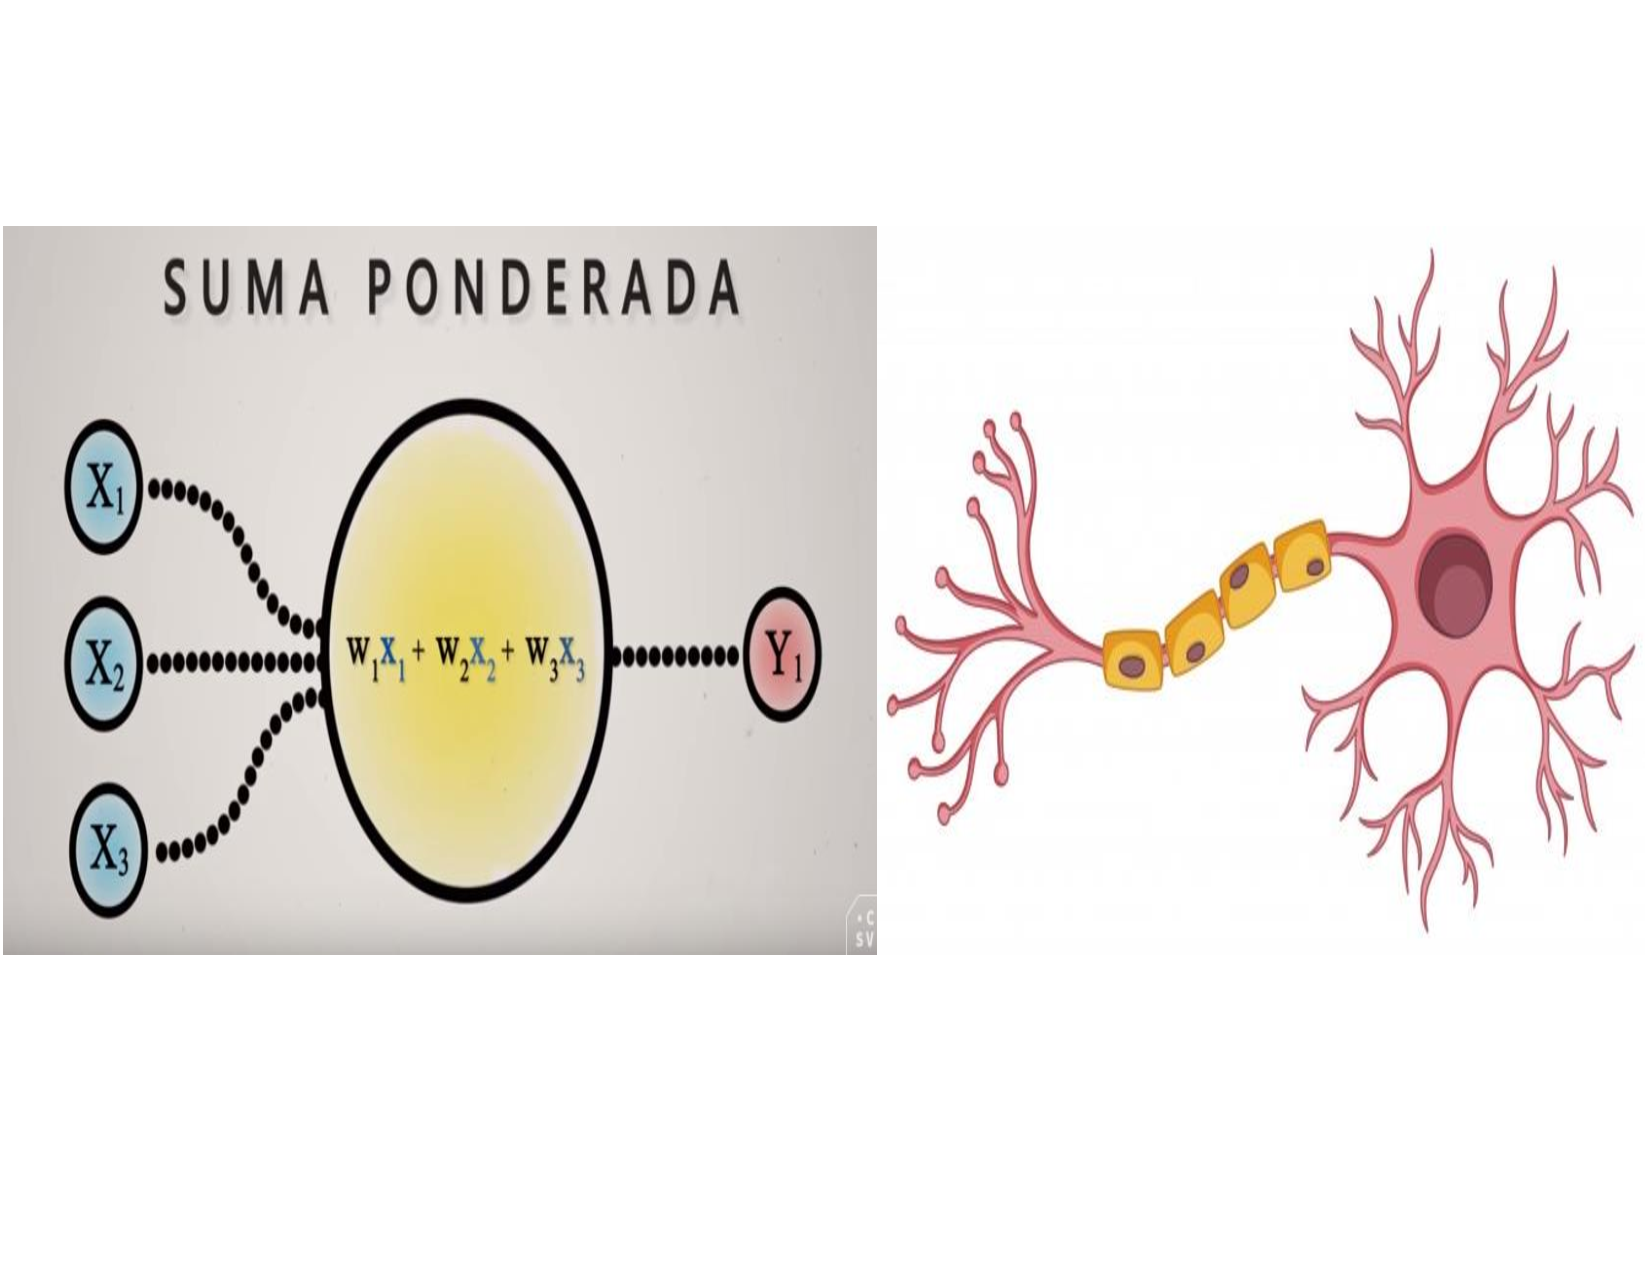
\includegraphics[scale=0.33]{FigurasUV/RN1.pdf}
\end{figure}
\end{frame}

\begin{frame}{¿Qué son las redes neuronales?}
Una regresión separa con una linea recta grupos de puntos:

\begin{figure}[h!]
  \centering
  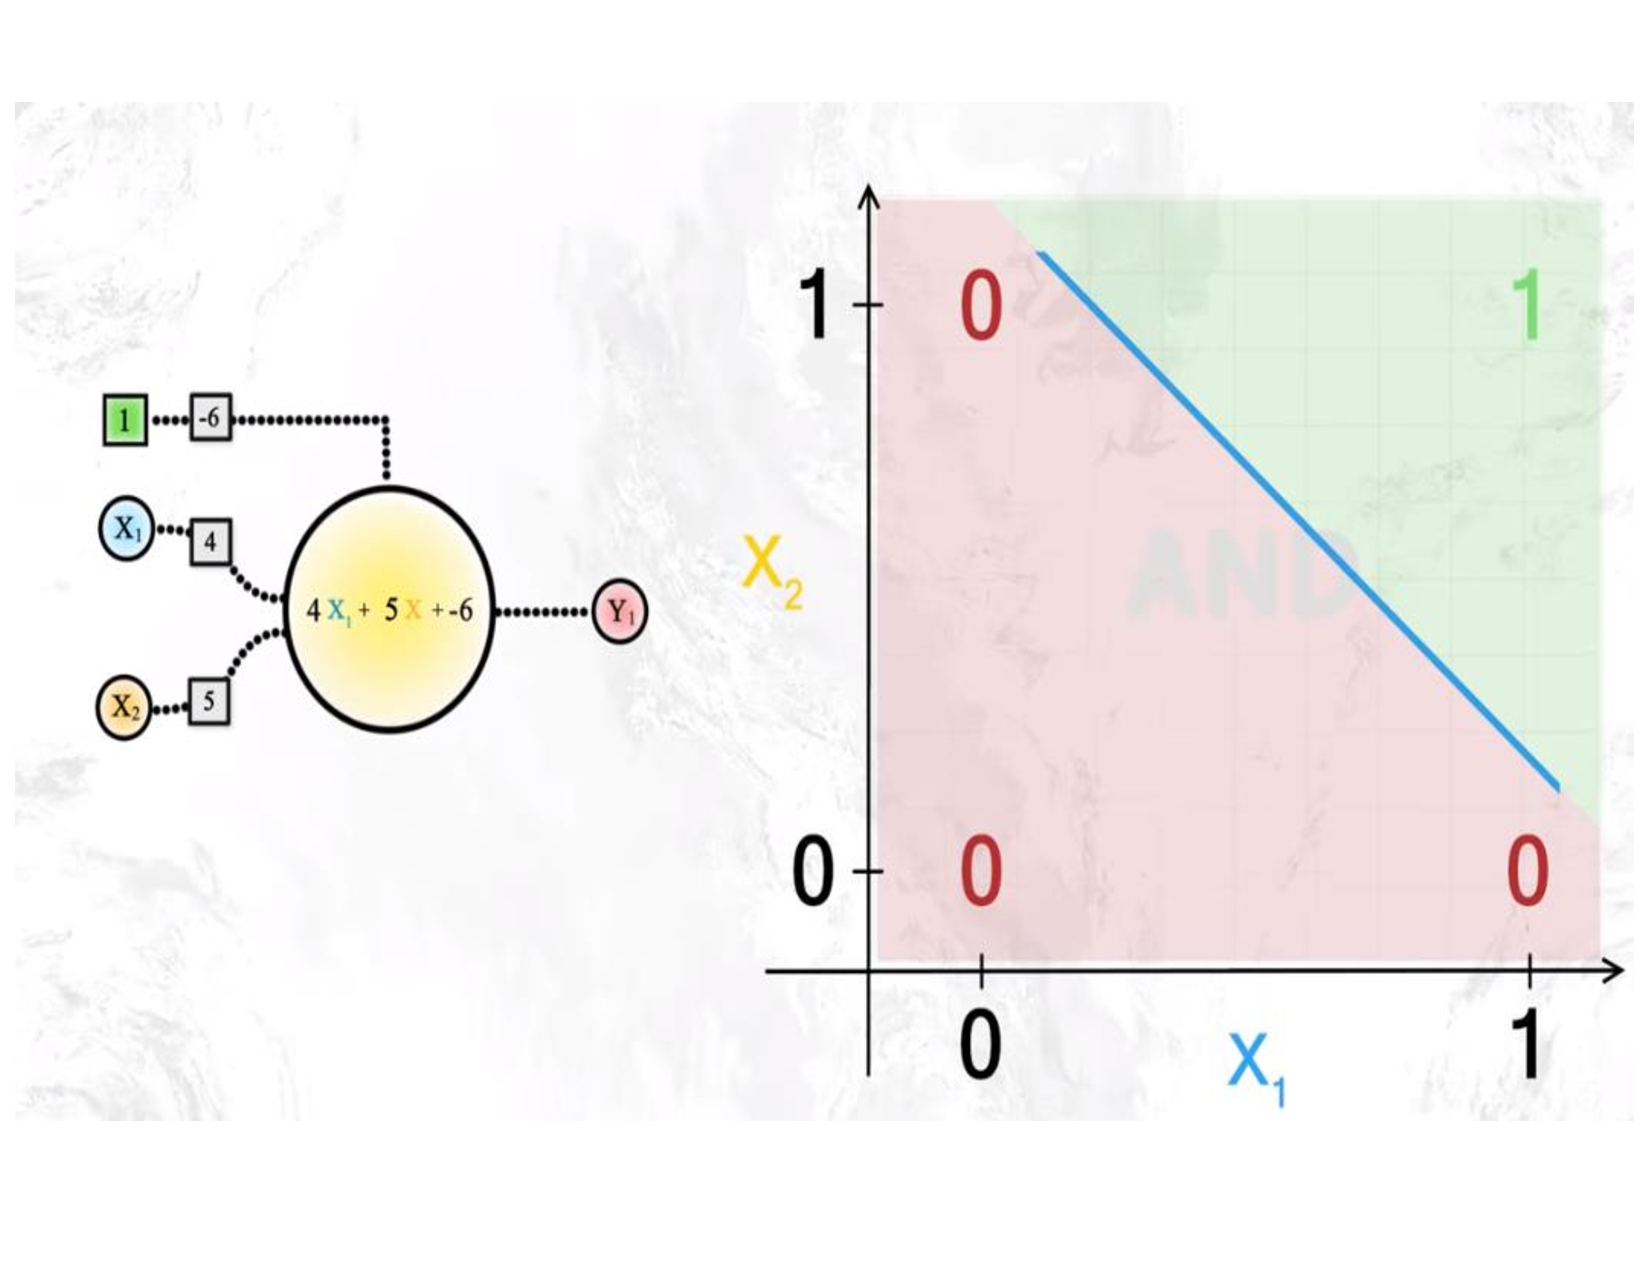
\includegraphics[scale=0.33]{FigurasUV/RN2.pdf}
\end{figure}

\end{frame}

\begin{frame}{¿Qué son las redes neuronales?}

\begin{figure}[h!]
  \centering
  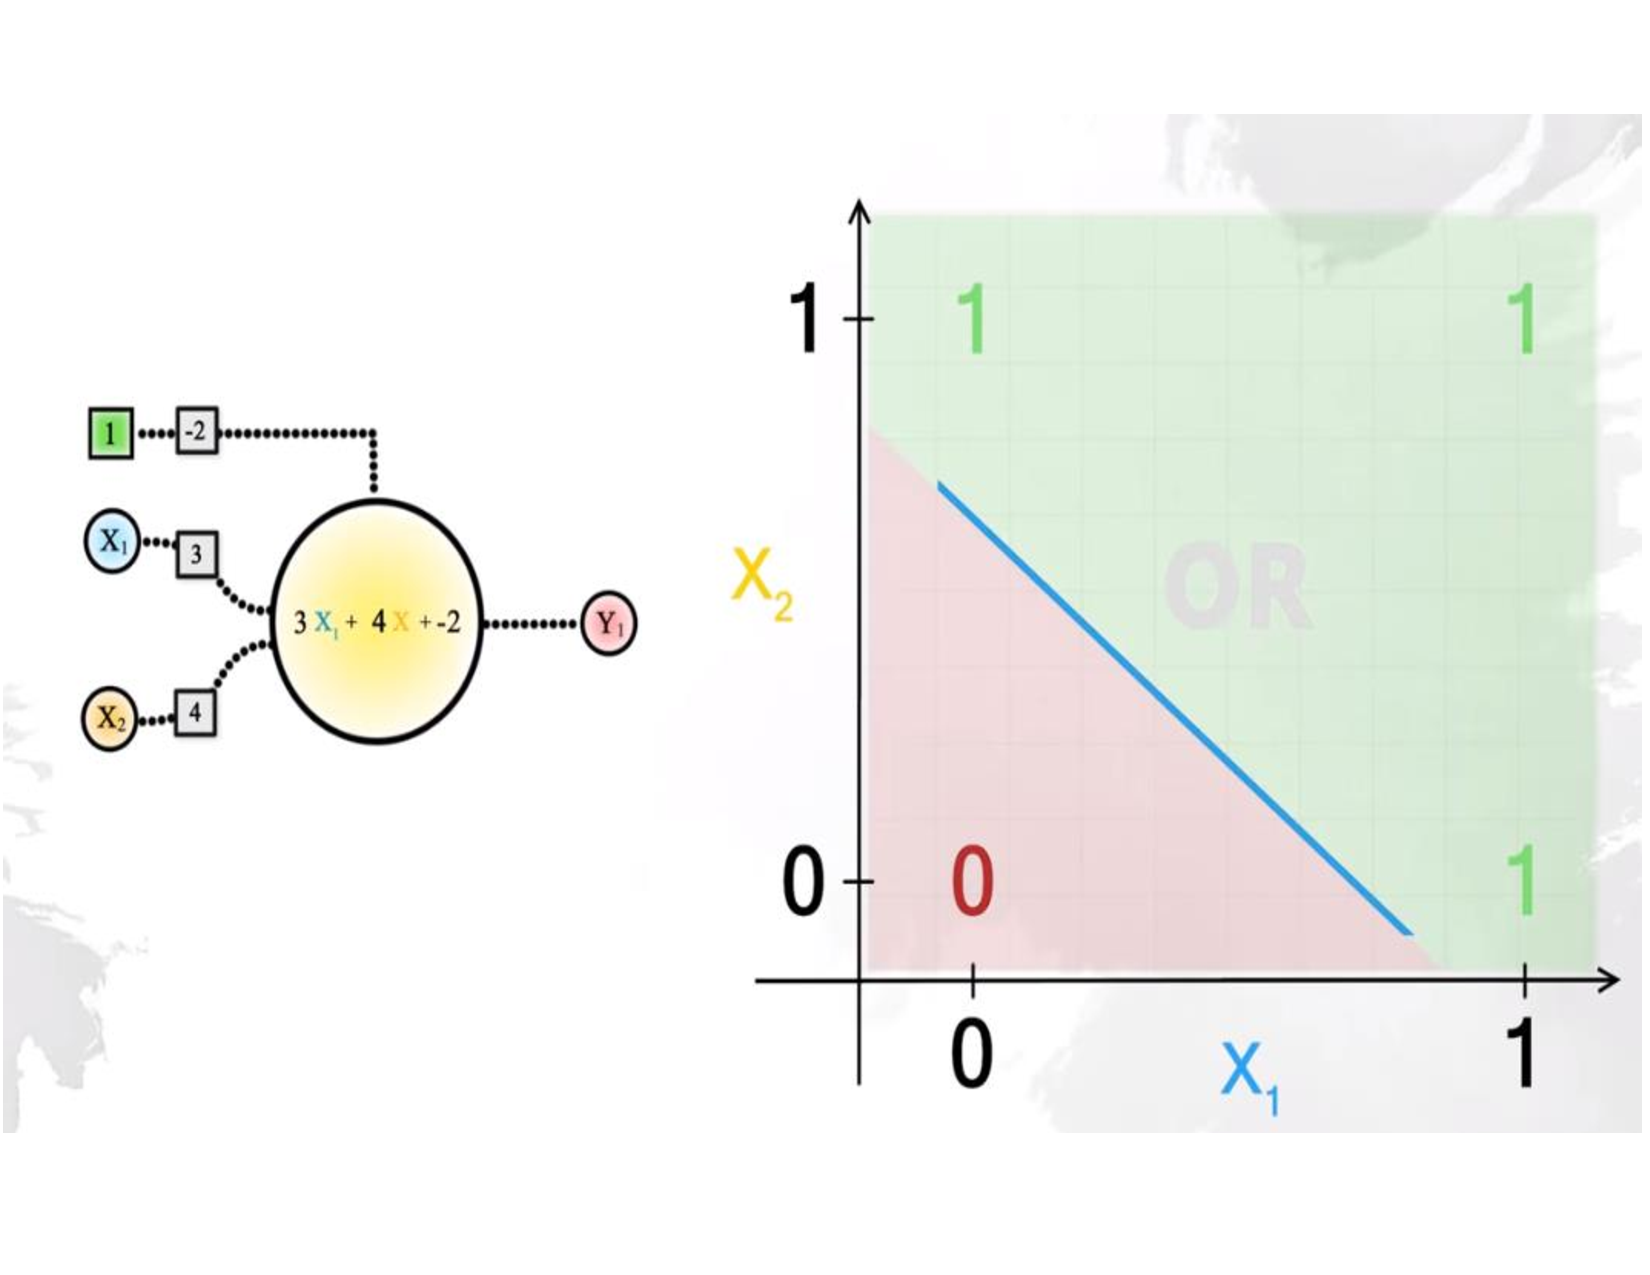
\includegraphics[scale=0.33]{FigurasUV/RN3.pdf}
\end{figure}

\end{frame}

\begin{frame}{¿Qué son las redes neuronales?}
¿Qué sucede cuando no es posible separar una nube de puntos con una linea?

\begin{figure}[h!]
  \centering
  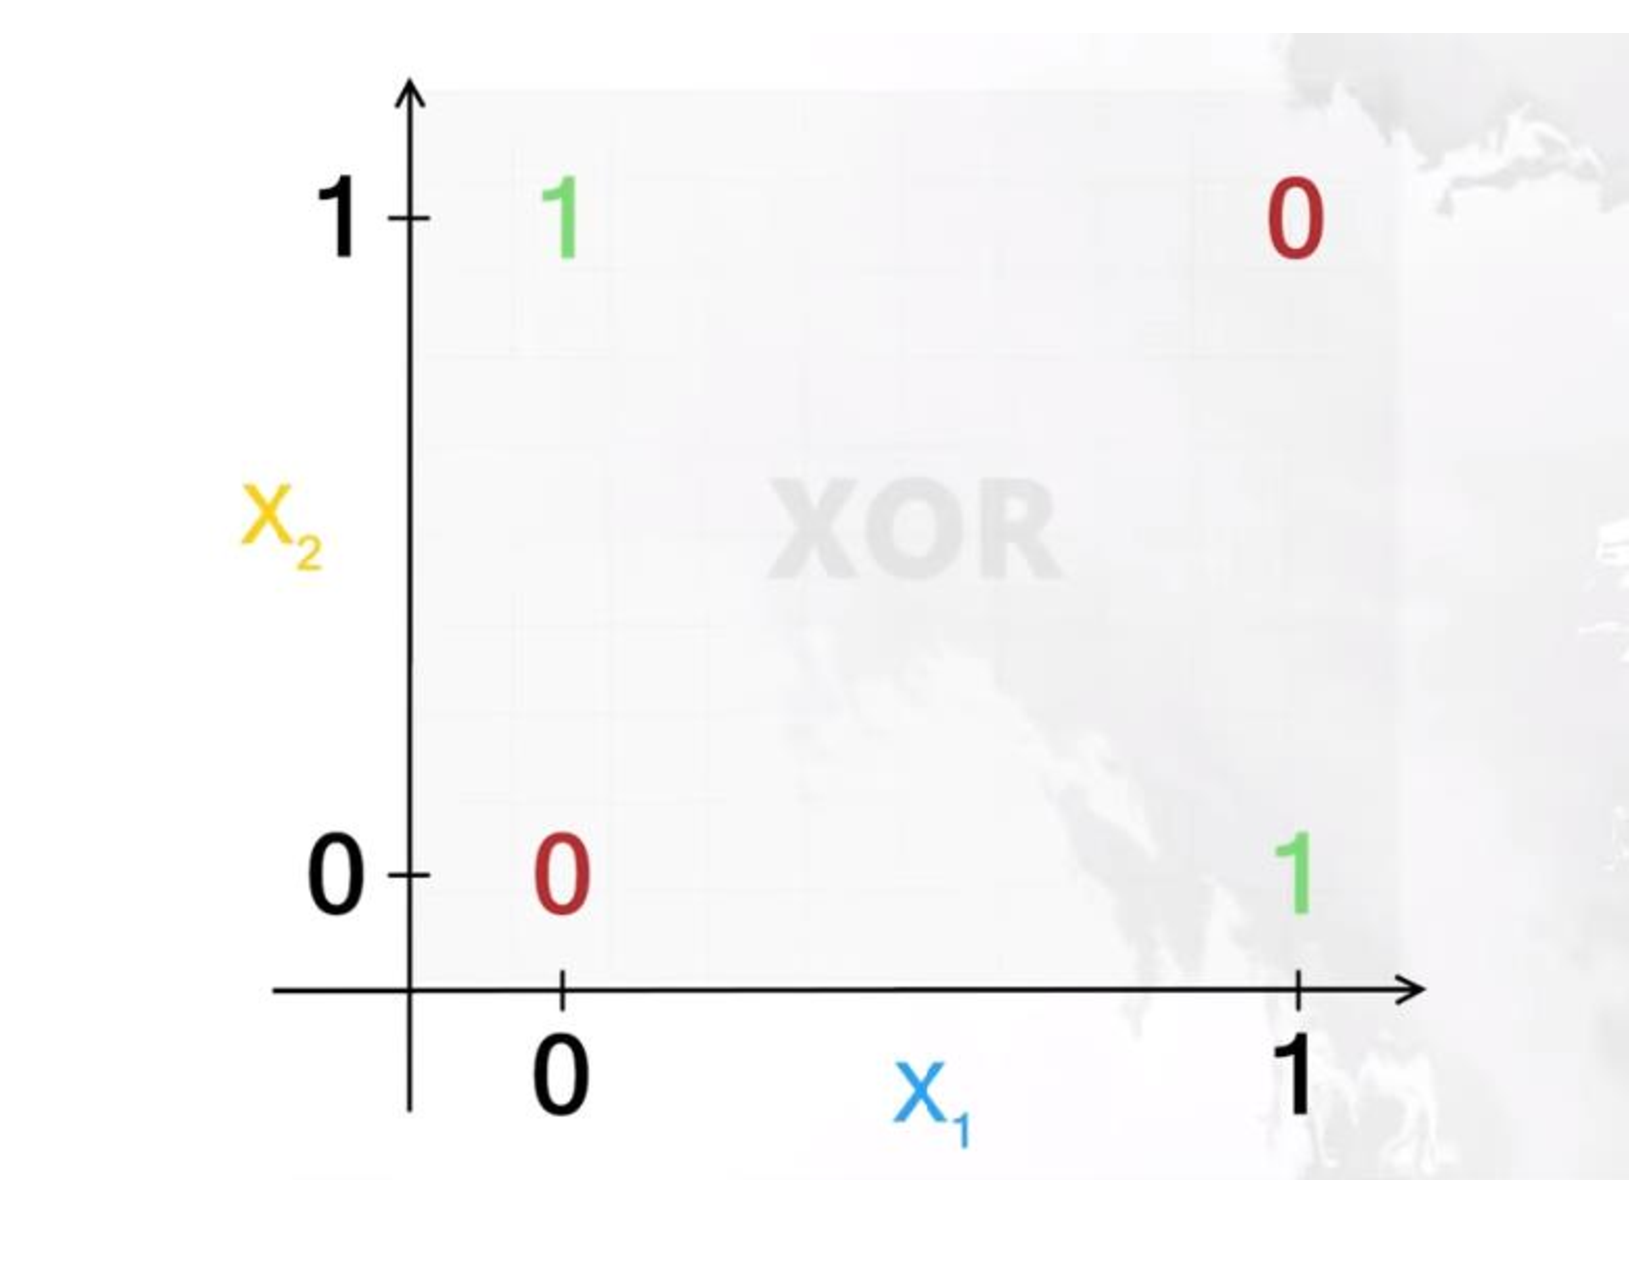
\includegraphics[scale=0.33]{FigurasUV/RN4.pdf}
\end{figure}

\end{frame}

\begin{frame}{¿Qué son las redes neuronales?}
Añadimos otra neurona:

\begin{figure}[h!]
  \centering
  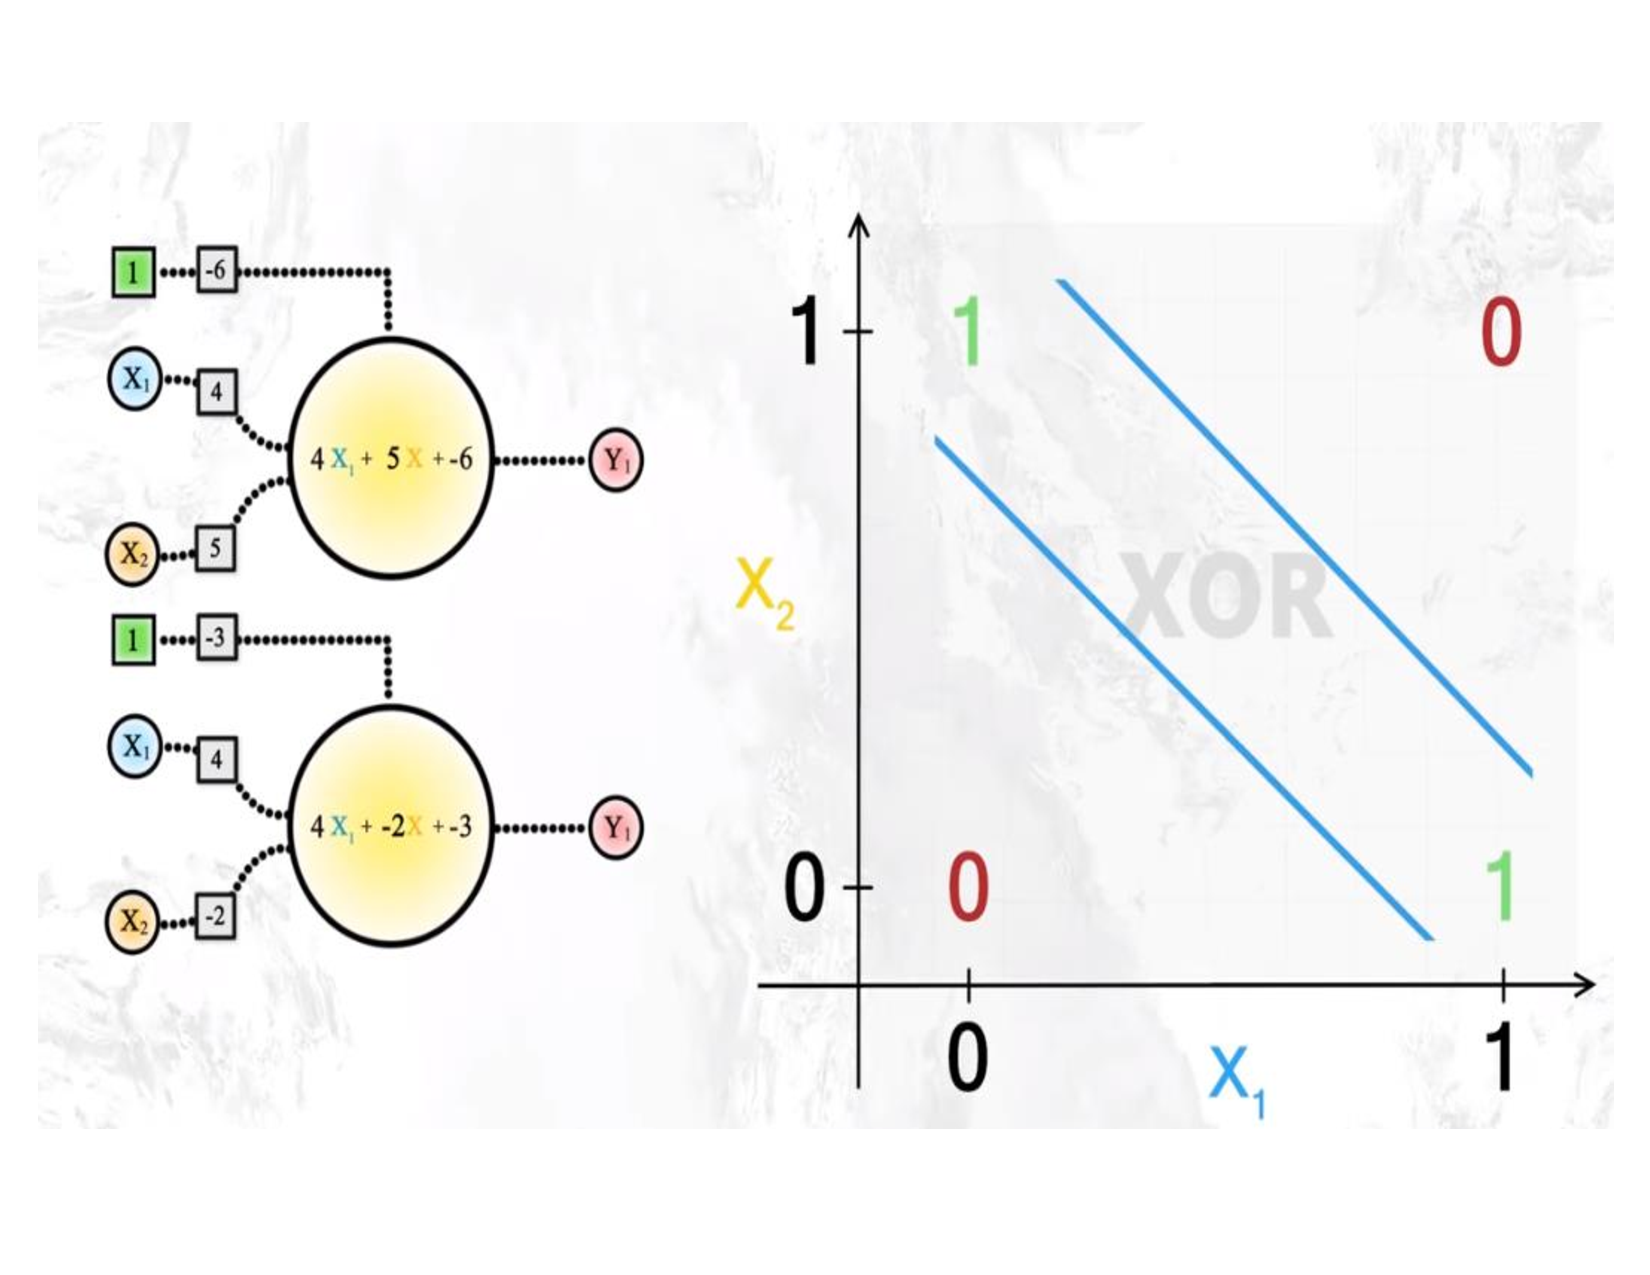
\includegraphics[scale=0.33]{FigurasUV/RN5.pdf}
  \caption{Neurona}
\end{figure}

\end{frame}

\begin{frame}{¿Qué son las redes neuronales?}
Si añadimos más:

\begin{figure}[h!]
  \centering
  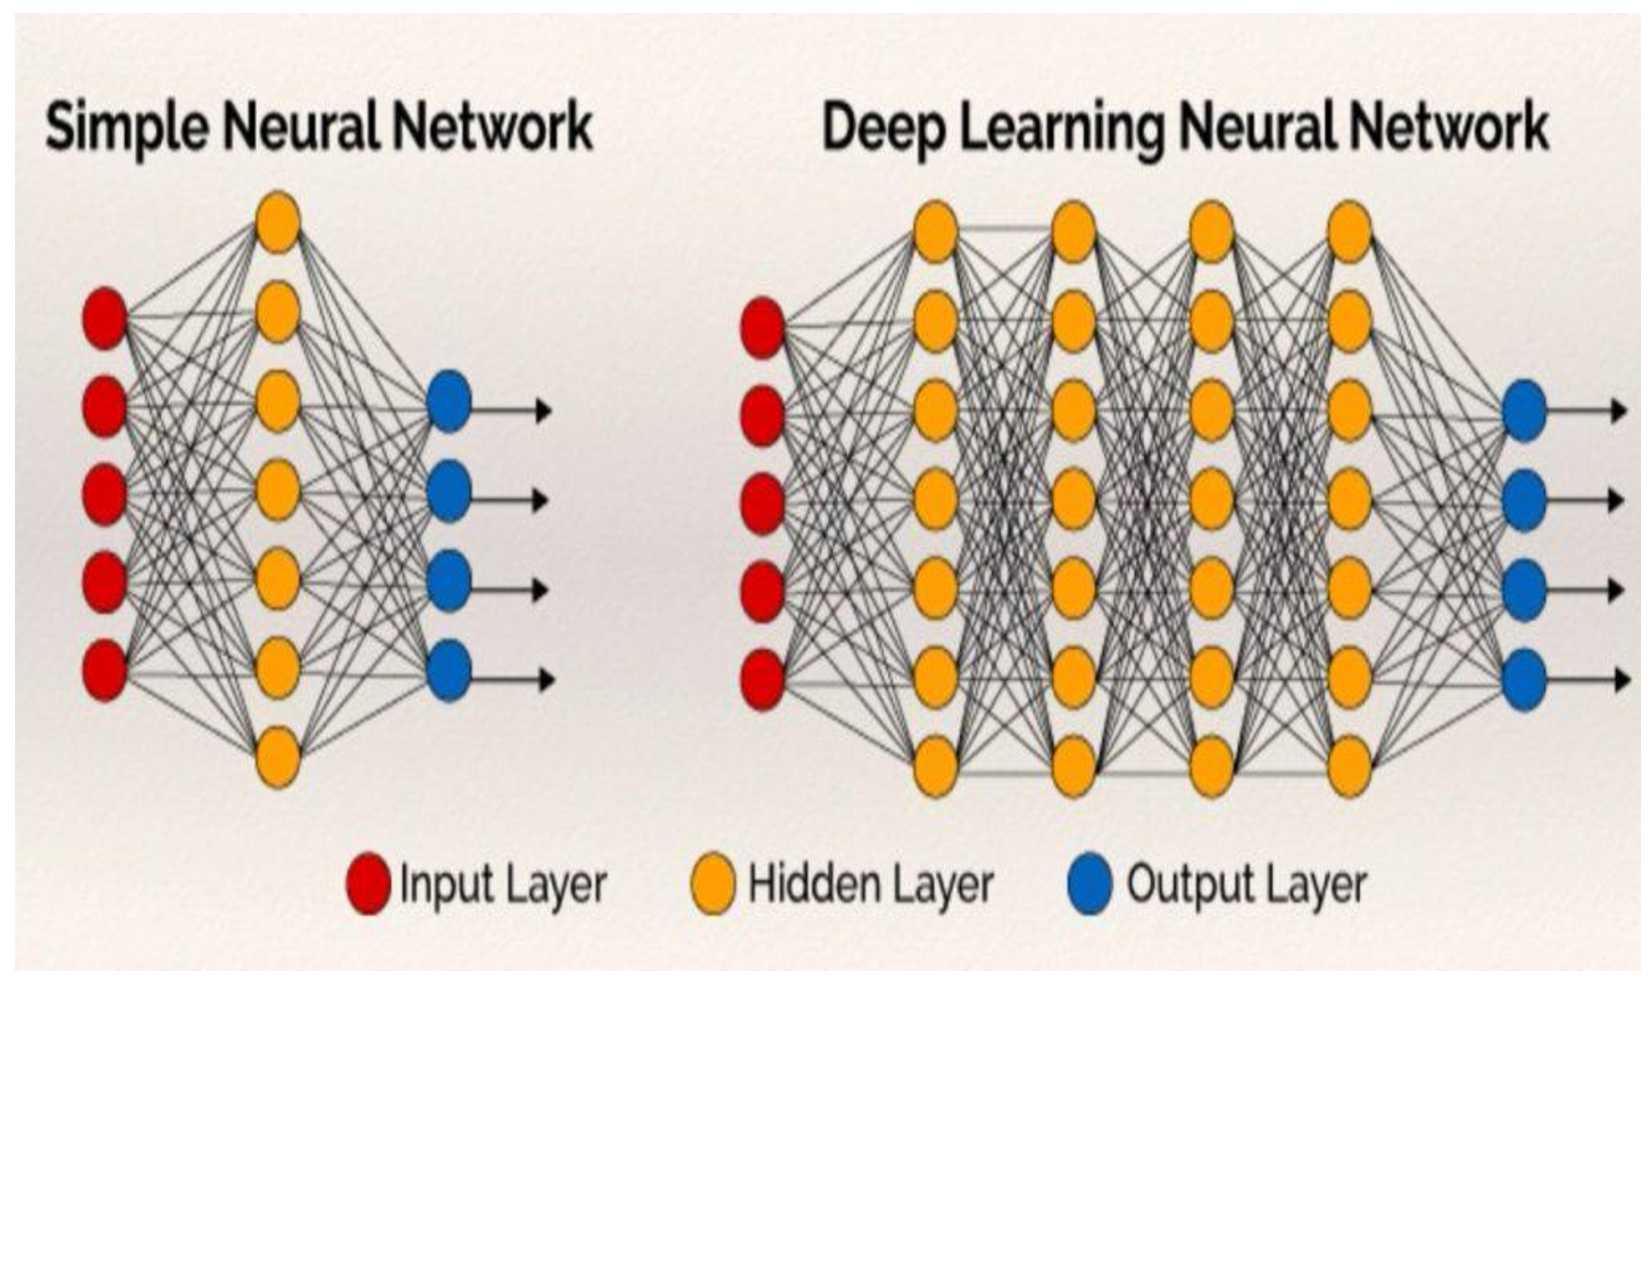
\includegraphics[scale=0.33]{FigurasUV/Red1.pdf}
  \caption{Neurona}
\end{figure}

\end{frame}

\begin{frame}{¿Qué son las redes neuronales?}
Una red neuronal está compuesta por neuronas o
nodos de procesamiento, y estos a su vez están divididos en grupos que se llaman ``capas''. Existen
3 tipos de capas: capas de entrada, capas ocultas y capas de salida; las conexiones se establecen
entre los nodos de cada capa adyacente, la capa de entrada está formada por nodos de entrada,
que reciben la información directamente del exterior; mientras que la capa de salida representa la
respuesta de la red a una entrada dada, siendo esta información transferida al exterior.

\end{frame}

\begin{frame}{¿Qué son las redes neuronales?}
Una red neuronal también la podemos ver de la siguiente forma:
$$a_l=g(\omega_{\ell0}^{(1)}+\sum_{j=1}^{p} \omega_{\ell j}^{(1)}X_j)$$
Donde, $a_l$ es la conexión a la capa de entrada a través de un vector de parámetros o pesos $\omega_{\ell j}^{(1)}$ (El (1) hace referencia a el numero de la capa en este caso seria la primera y $\ell j$ hace referencia a la $j-esima$ variable y la $\ell-esima$ unidad). Los términos $\omega_{\ell0}^{(1)}$ son los sesgos o interceptos y la función $g$ es llamada función de activación,usualmente se utilizan funciones sigmoides en las capas de salidas ya que estas arrojan valores entre 0 y 1 ($g=\frac{1}{(1-e^{-t})}$) y en el resto de capas se suelen utilizar funciones ReLU (Rectified Linear Unit Function).

 
\end{frame}


\section{¿Cómo funcionan?}
\begin{frame}{¿Cómo funcionan?}
Al poner dos neuronas de forma secuencial, una de ellas recibe la información procesada por la neurona anterior, esto trae una ventaja muy importante para el aprendizaje
de la red y es que la red podrá aprender conocimiento jerarquizado, lo que sería en palabras simples,
que mis neuronas en las primeras capas sean capaces de procesar cosas simples y mis neuronas en
capas posteriores hagan procesos más complejos con la información suministrada por las primeras
capas.
\end{frame}

\begin{frame}{¿Cómo funcionan?}
Un ejemplo, un fin de semana perfecto es:

\begin{figure}[h!]
  \centering
  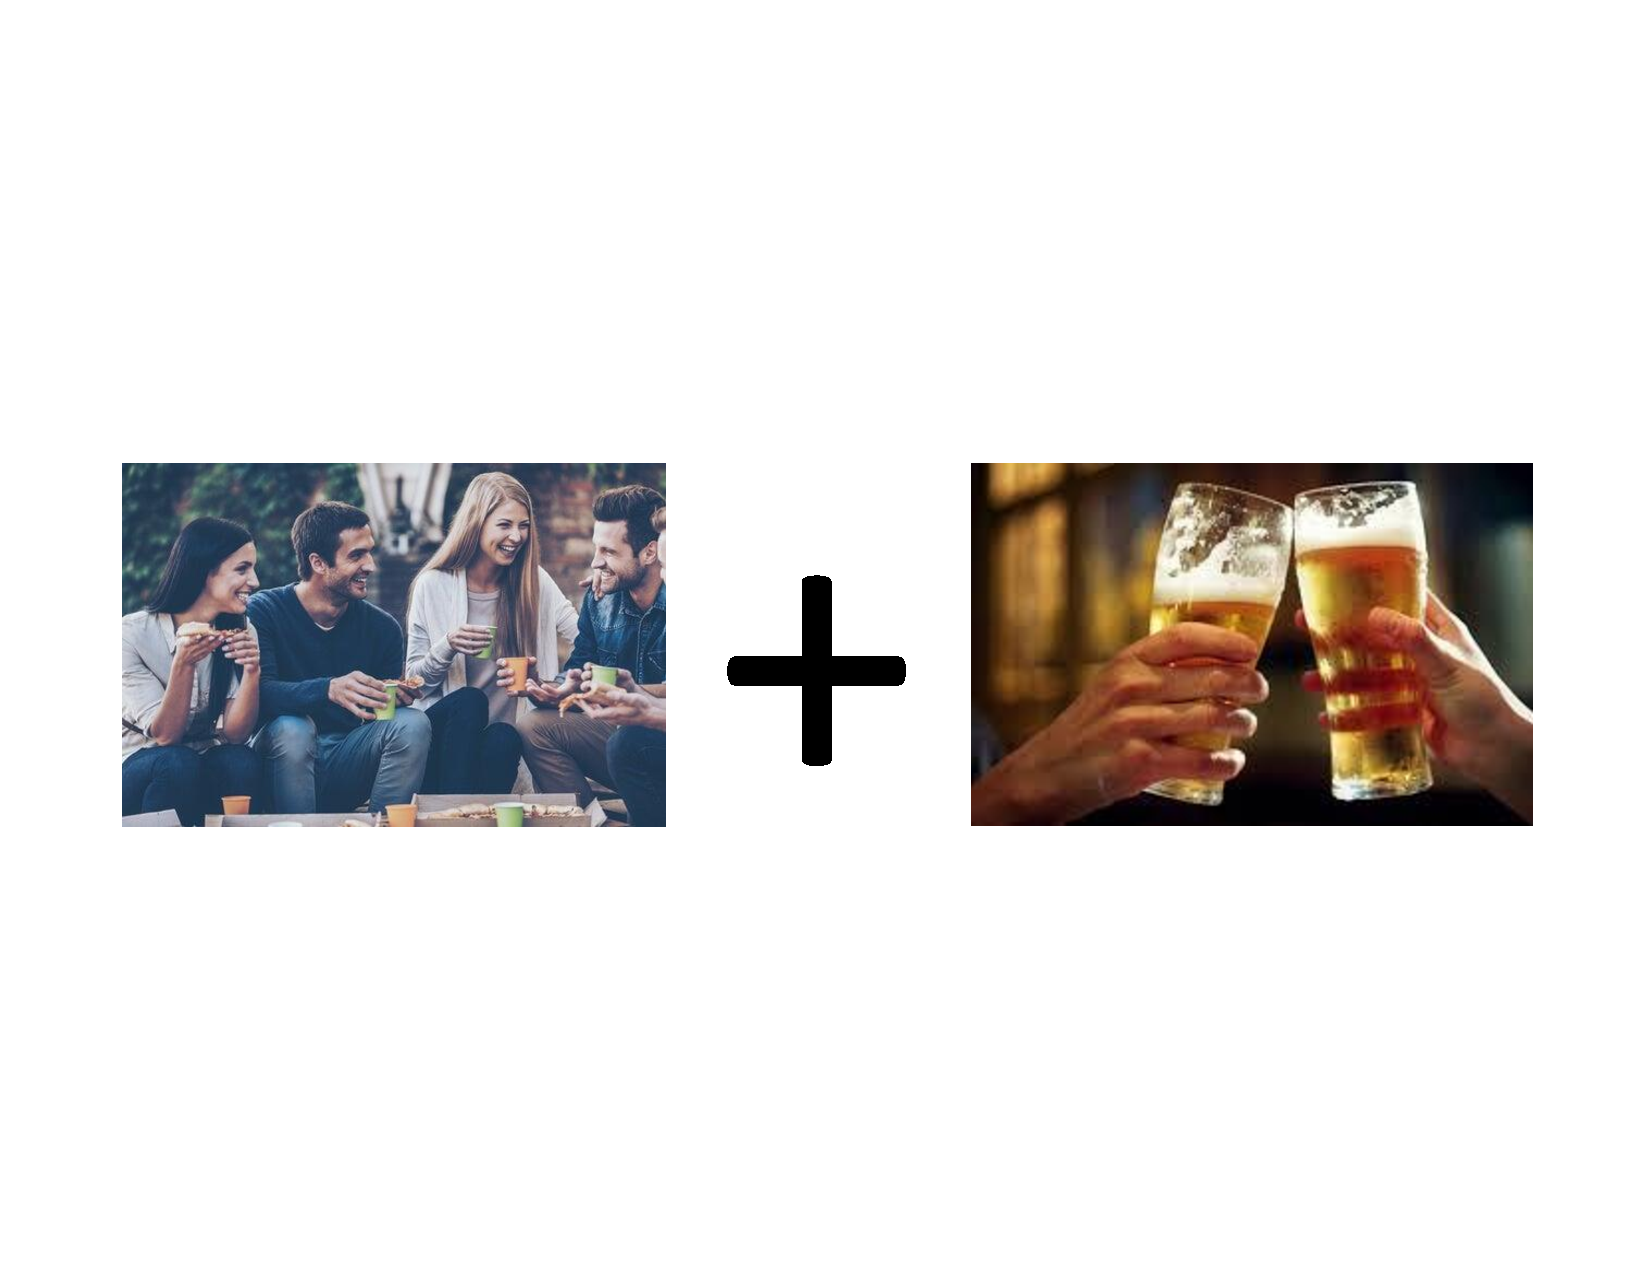
\includegraphics[scale=0.33]{FigurasUV/RN6.pdf}
  \caption{Neurona}
\end{figure}

\end{frame}

\begin{frame}{¿Cómo funcionan?}
No es posible que sea perfecto si una de estas condiciones no se cumple; con una regresión simple podría modelar si mi fin de semana va a ser perfecto o no.

\begin{figure}[h!]
  \centering
  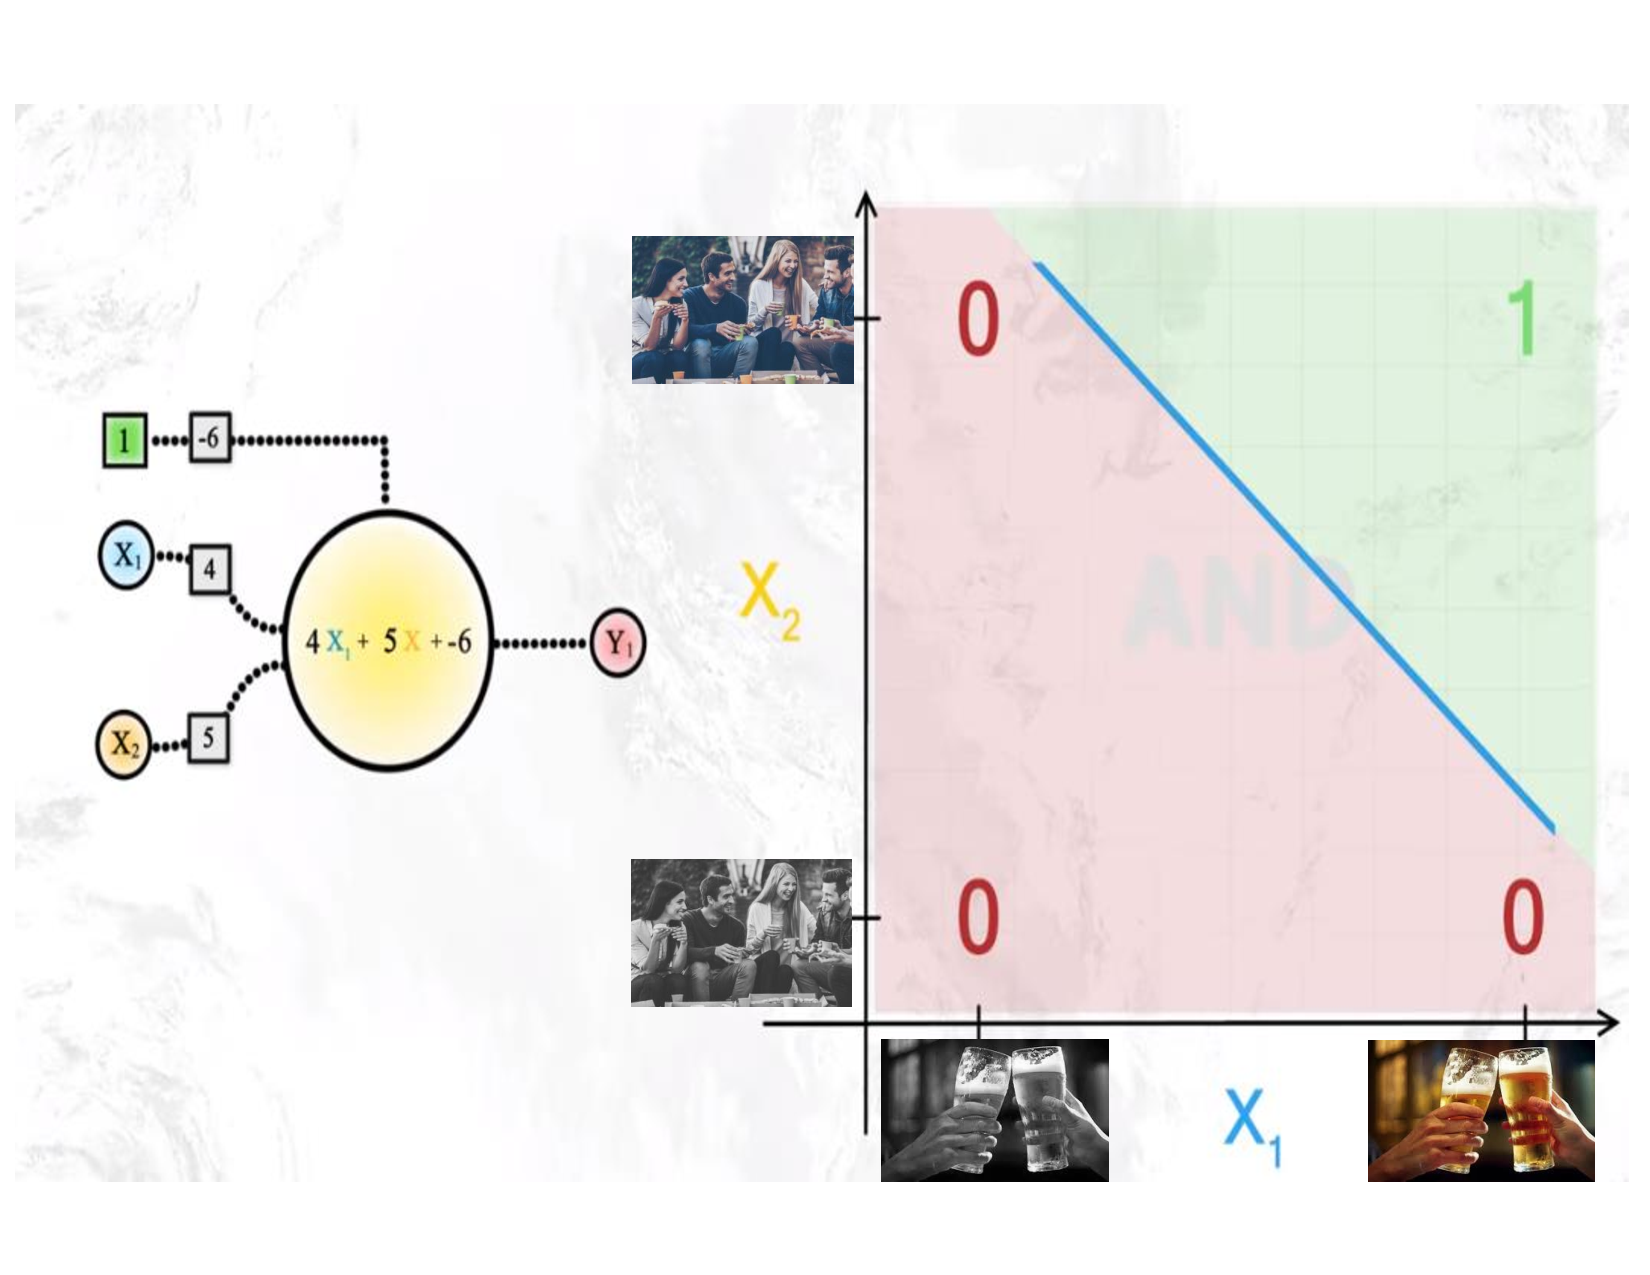
\includegraphics[scale=0.33]{FigurasUV/EJ1.pdf}
  \caption{Neurona}
\end{figure}

\end{frame}

\begin{frame}{¿Cómo funcionan?}
Pero si mi objetivo final es conocer algo más complejo como, ¿cuál sera mi calificación en el examen final del lunes?. A lo mejor existen otras 2 variables relacionadas, interés por la materia y dificultad del examen.

\begin{figure}[h!]
  \centering
  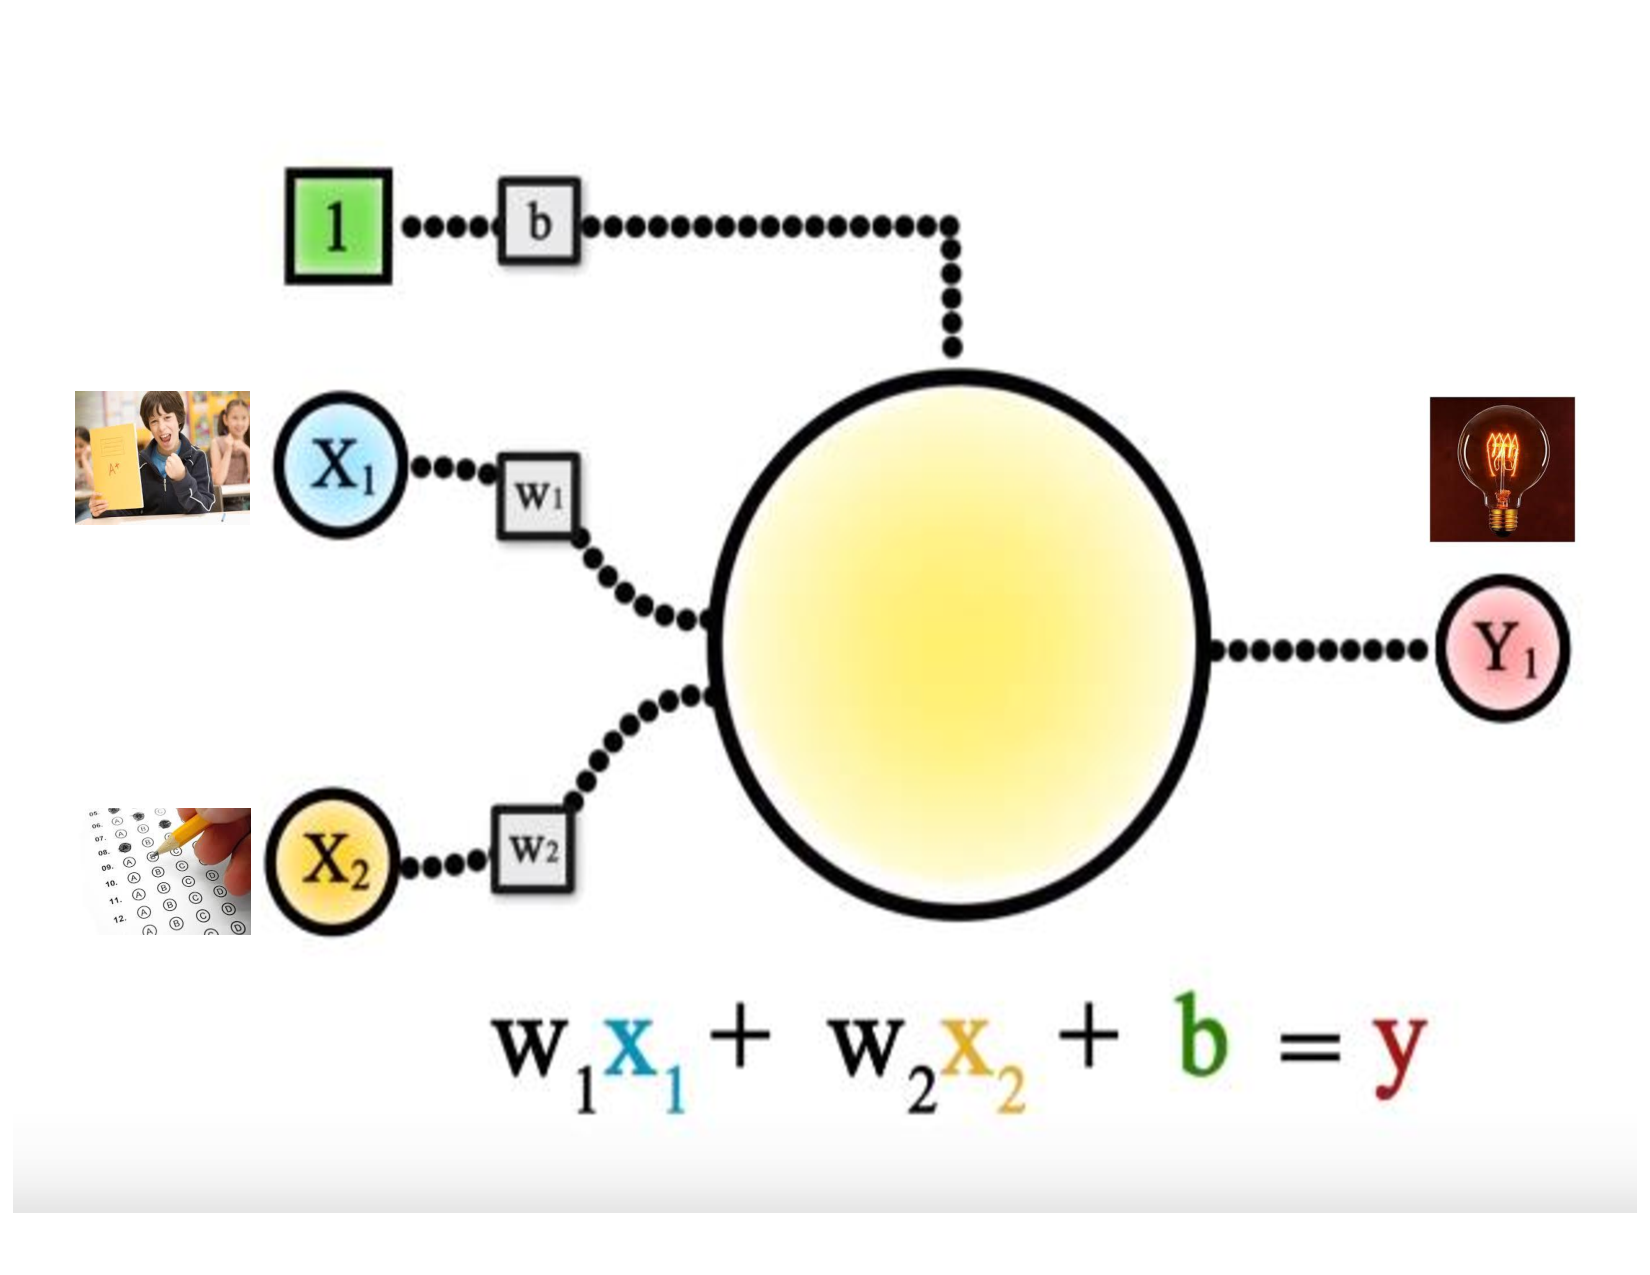
\includegraphics[scale=0.33]{FigurasUV/RN7.pdf}
  \caption{Neurona}
\end{figure}

\end{frame}

\begin{frame}{¿Cómo funcionan?}
Uniendo ambas neuronas obtenemos una posible arquitectura de  red neuronal:
\begin{figure}[h!]
  \centering
  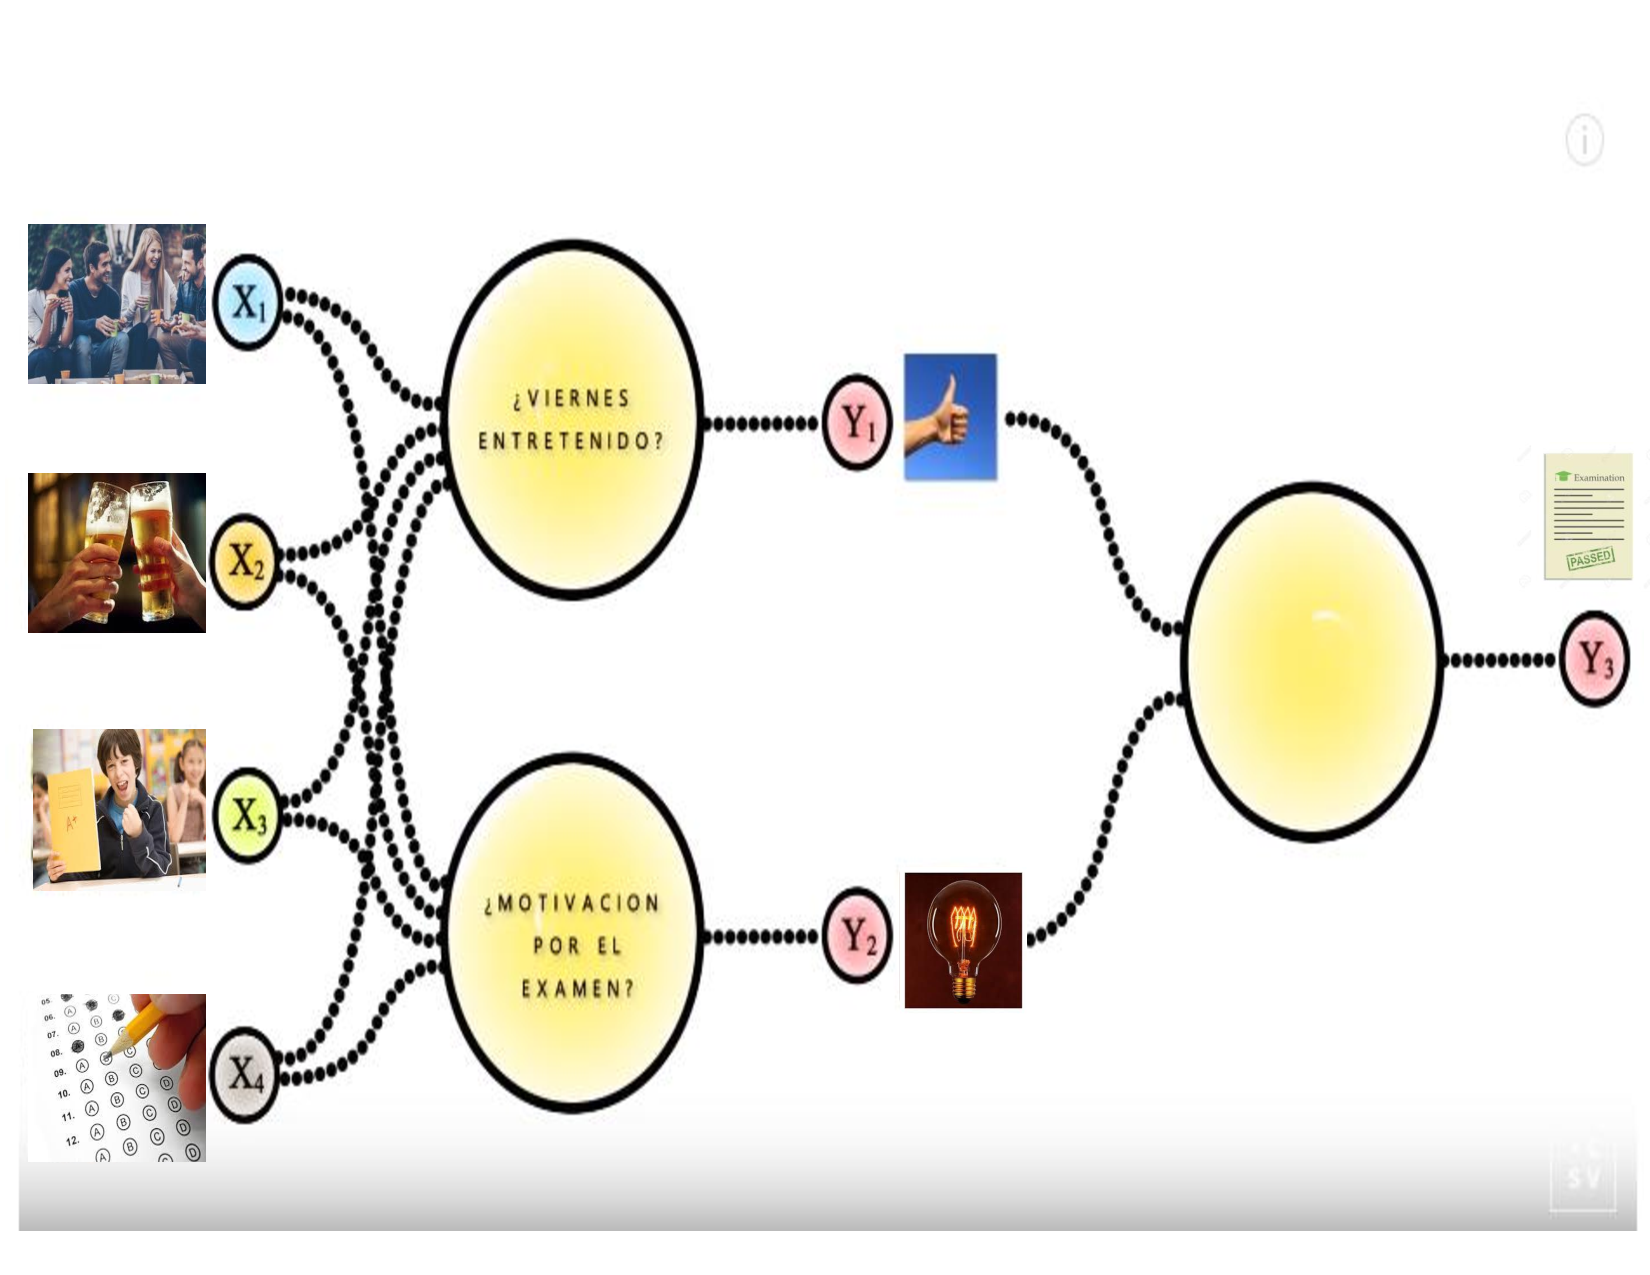
\includegraphics[scale=0.33]{FigurasUV/EJ2.pdf}
  \caption{Neurona}
\end{figure}

\end{frame}

\begin{frame}{¿Cómo funcionan?}
Mi red puede distinguir que estudiantes van a aprobar el examen del lunes; si su motivación por el examen es baja y su fin de semana fue perfecto, posiblemente van a estudiar poco y reprobarán el examen. De esta manera jerarquizada mi red puede generar conocimiento complejo, entre más neuronas y capas sean agregadas, más complejo será. A esta manera de aprender se le llama ``Deep Learning''.

\end{frame}


\begin{frame}{¿Cómo funcionan?}
Para conseguir este aprendizaje profundo en nuestra red hay que conectar múltiples neuronas de forma secuencial, como lo que realiza cada neurona es una regresión lineal, matemáticamente estamos sumando múltiples regresiones lineales.

\begin{figure}[h!]
  \centering
  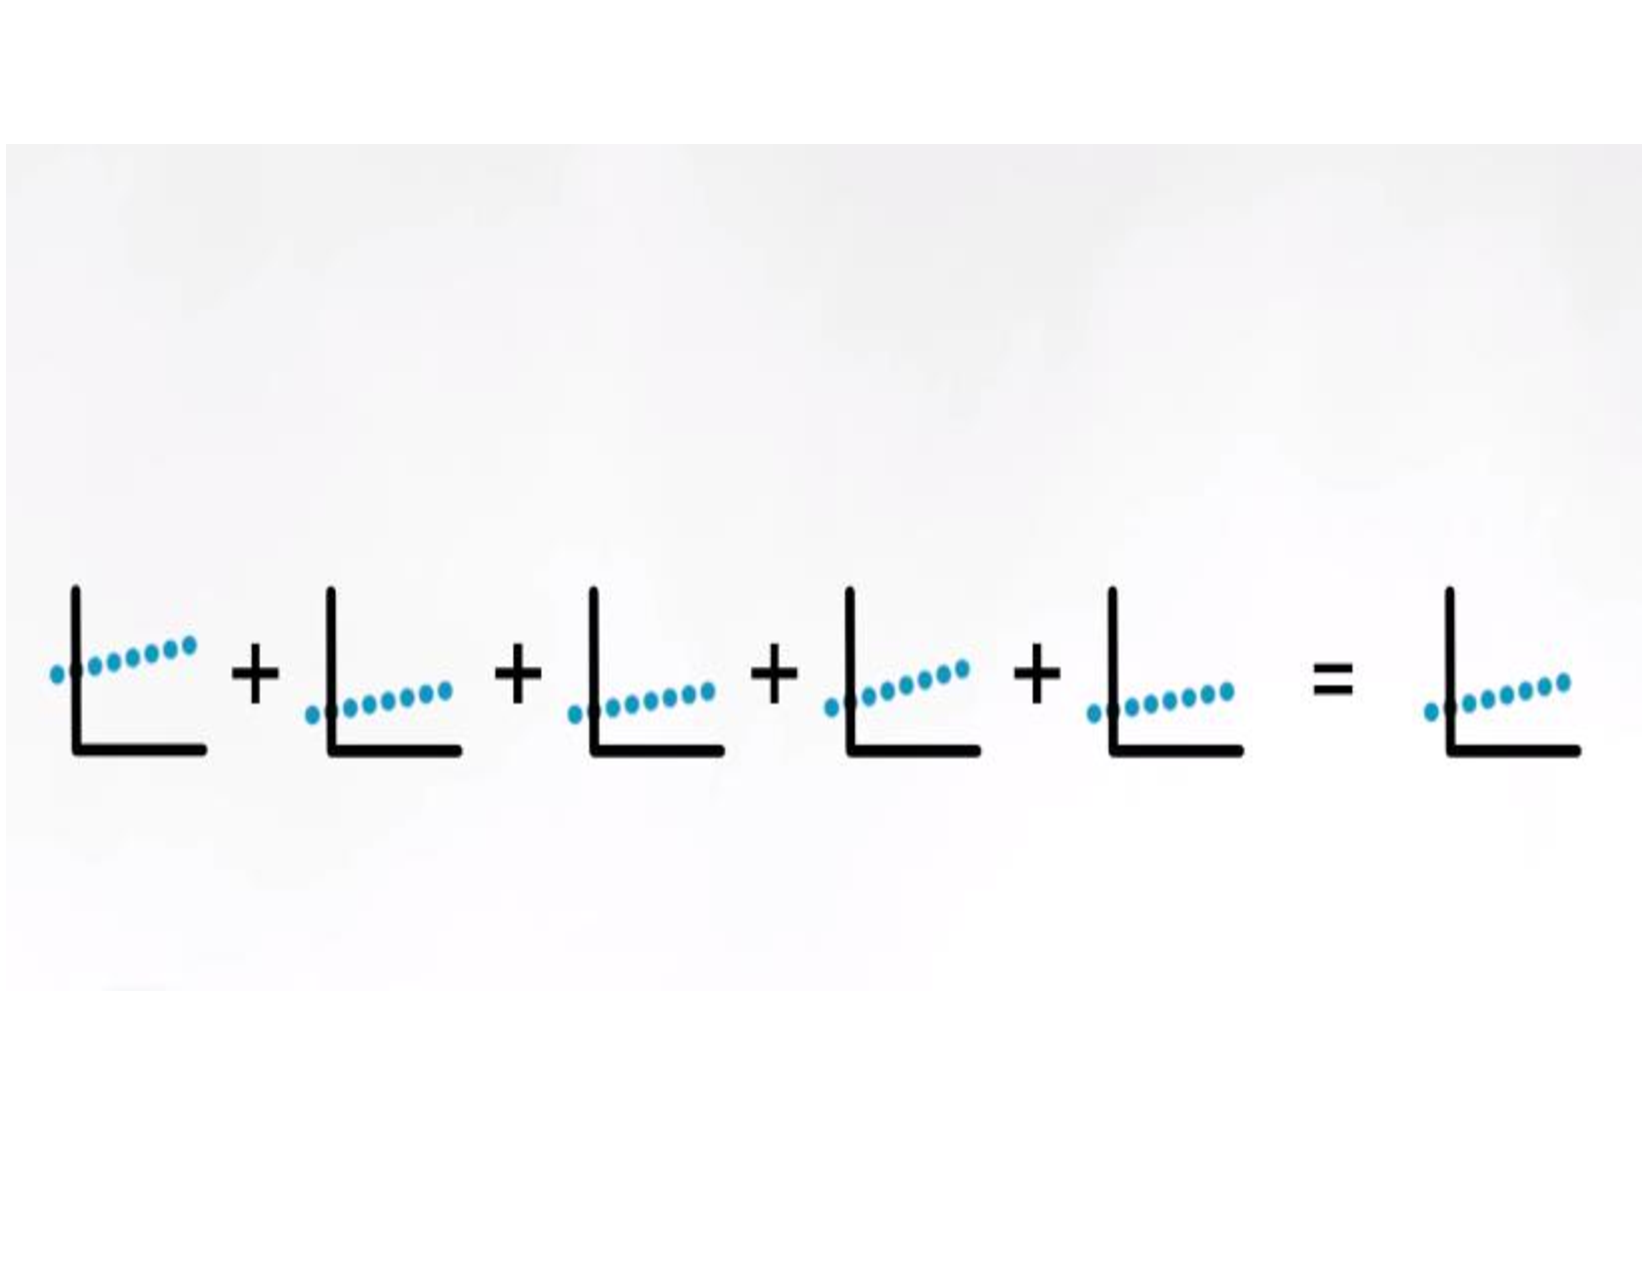
\includegraphics[scale=0.35]{FigurasUV/RN8.pdf}
  \caption{Neurona}
\end{figure}

\end{frame}

\begin{frame}{¿Cómo funcionan?}
Para que esto no suceda y nuestra red pueda aprender debemos adicionar deformaciones no lineales a nuestras regresiones; estas deformaciones se adicionan mediante la función de activación. 

\begin{figure}[h!]
  \centering
  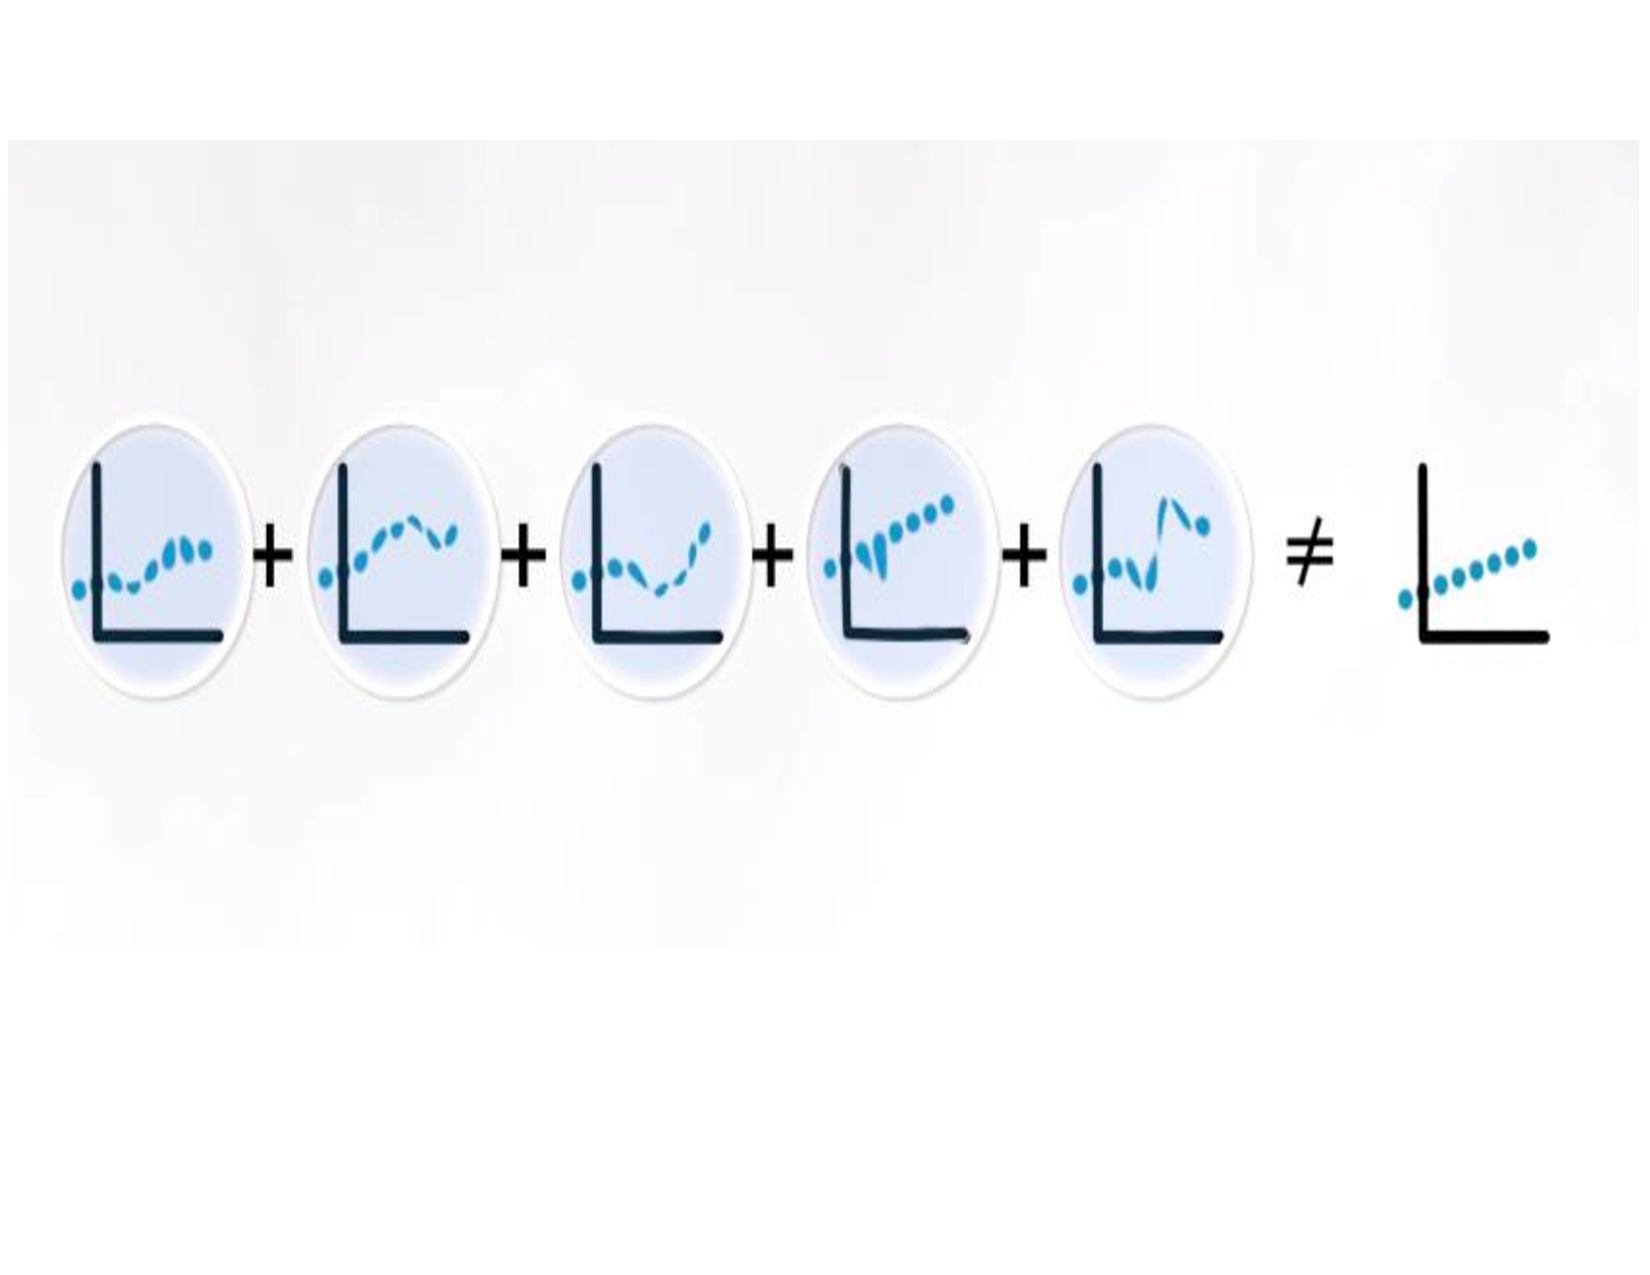
\includegraphics[scale=0.35]{FigurasUV/RN9.pdf}
  \caption{Neurona}
\end{figure}

\end{frame}
\section{Funciones de activación}
\begin{frame}{Funciones de activación}
Una función de activación añade deformaciones no lineales, de manera que mis valores de salida pasan primero por una determinada función, esto hace que mi red no colapse en una única regresión lineal. Estas deformaciones dependen de la función de activación utilizada, existen varios tipos, las más usadas son:
\end{frame}

\subsection{Función sigmoide}
\begin{frame}{Función sigmoide}
La función sigmoide denotada de la forma $G(x)=\frac{1}{(1-e^{-x})}$  hace que los valores muy altos se saturen en 1 y los valores bajos en 0 por lo tanto esta función añade dicha deformación no lineal y además representa muy bien probabilidades.

\begin{figure}[h!]
  \centering
  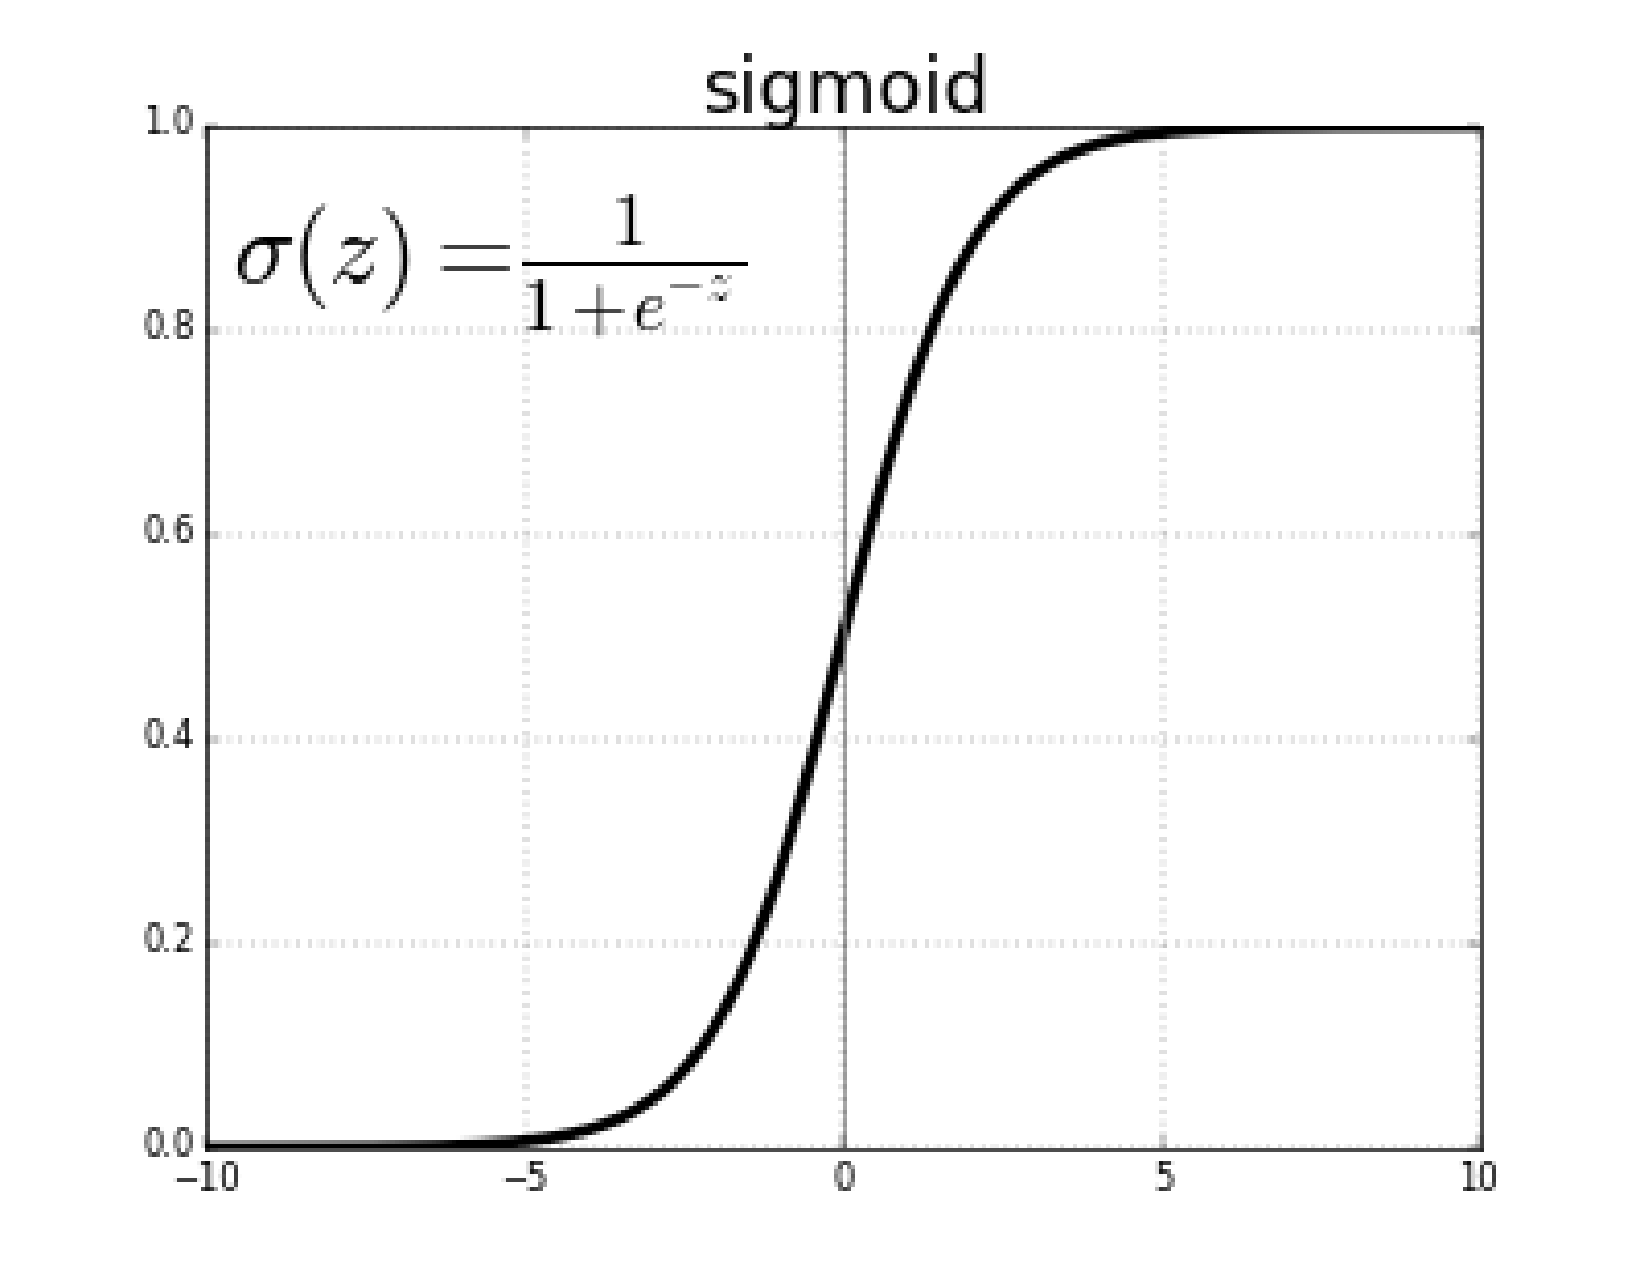
\includegraphics[scale=0.2]{FigurasUV/sigmoide.pdf}
  \caption{Función sigmoide}
\end{figure}


\end{frame}
\subsection{Función Tanh}
\begin{frame}{Función Tanh}
Similar a la función sigmoide está la función tangente hiperbólica, su forma es  similar a la sigmoide pero su rango varia entre -1 y 1 y está dada por $G(x)=tanh(x)=\frac{e^{x}-e^{-x}}{e^{x}+e^{-x}}$

\begin{figure}[h!]
  \centering
  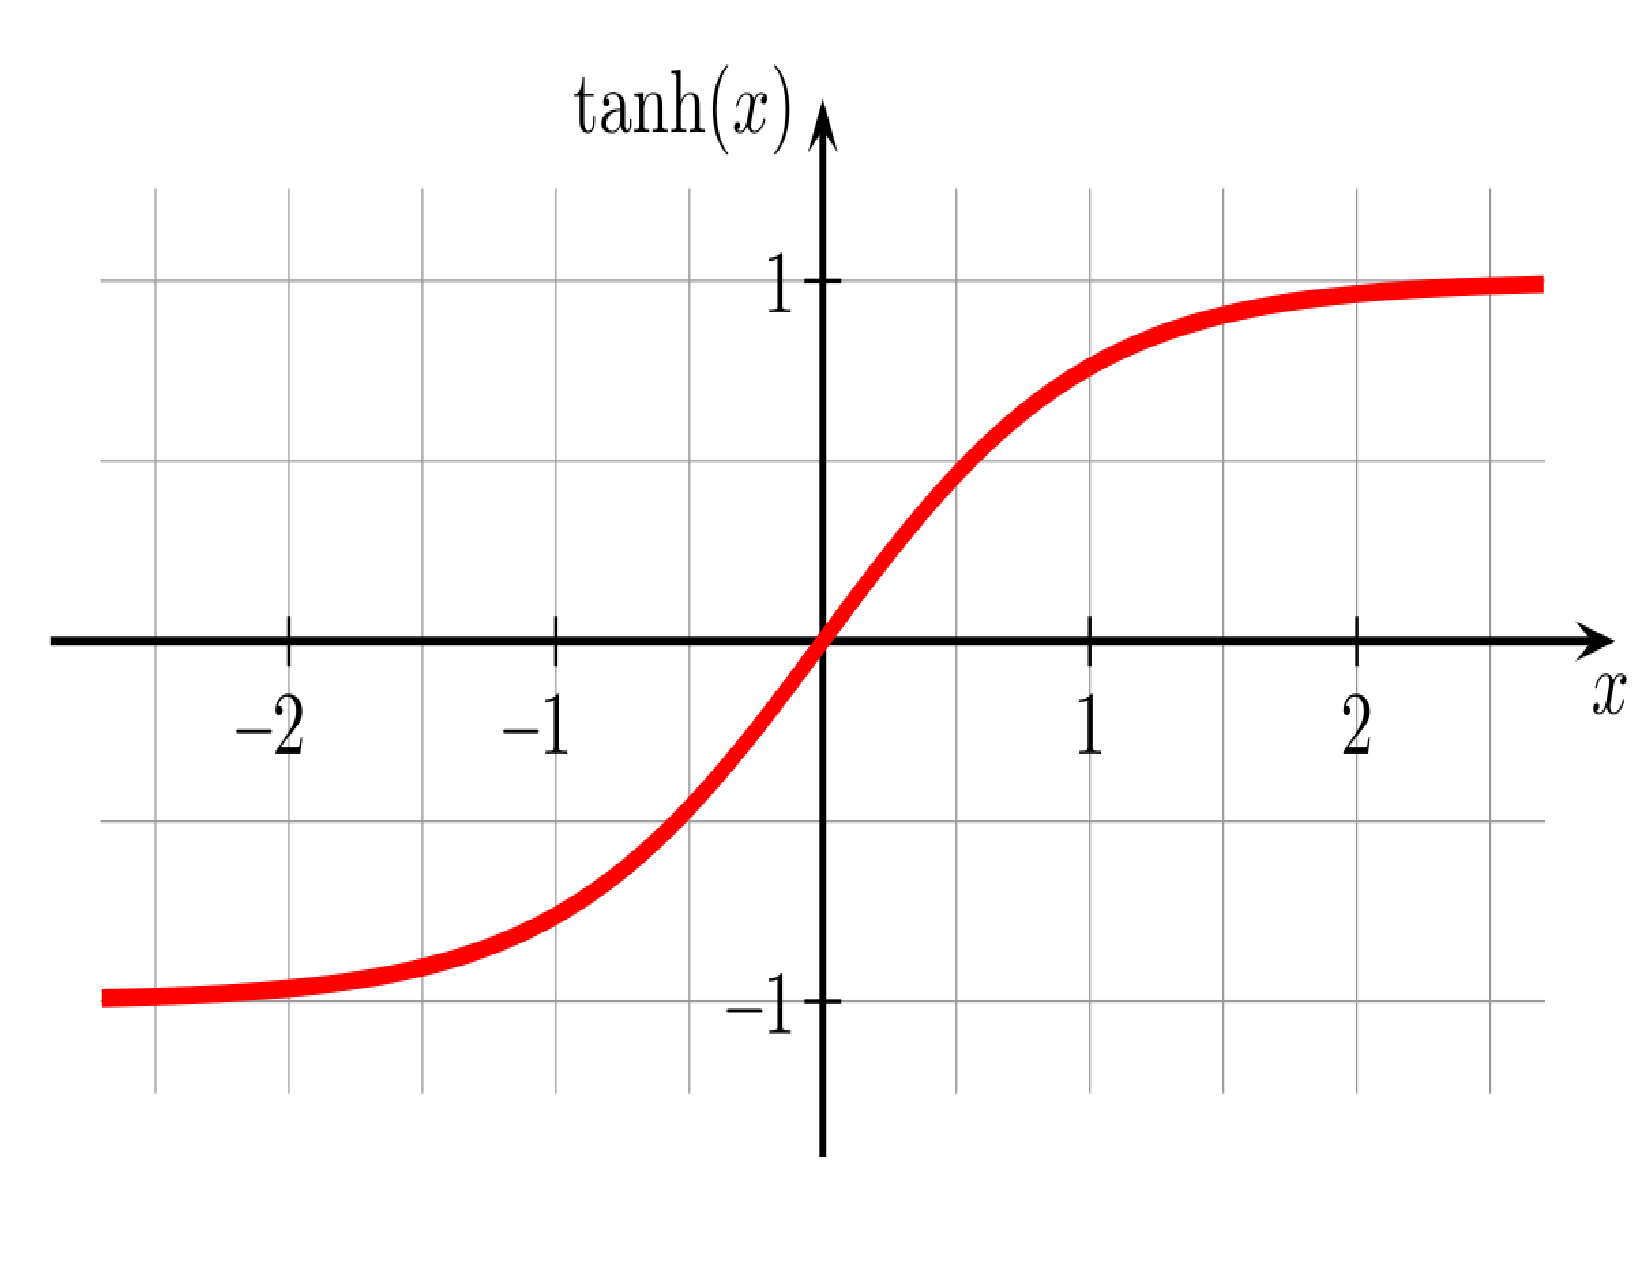
\includegraphics[scale=0.2]{FigurasUV/Tanh.pdf}
  \caption{Función Tanh}
\end{figure}

\end{frame}
\subsection{Función ReLU}
\begin{frame}{Función ReLU}
Esta función se comporta de forma lineal cuando es positiva y constante a 0 cuando el valor de entrada es negativo, se puede denotar como $G(x)=max(0,x)$

\begin{figure}[h!]
  \centering
  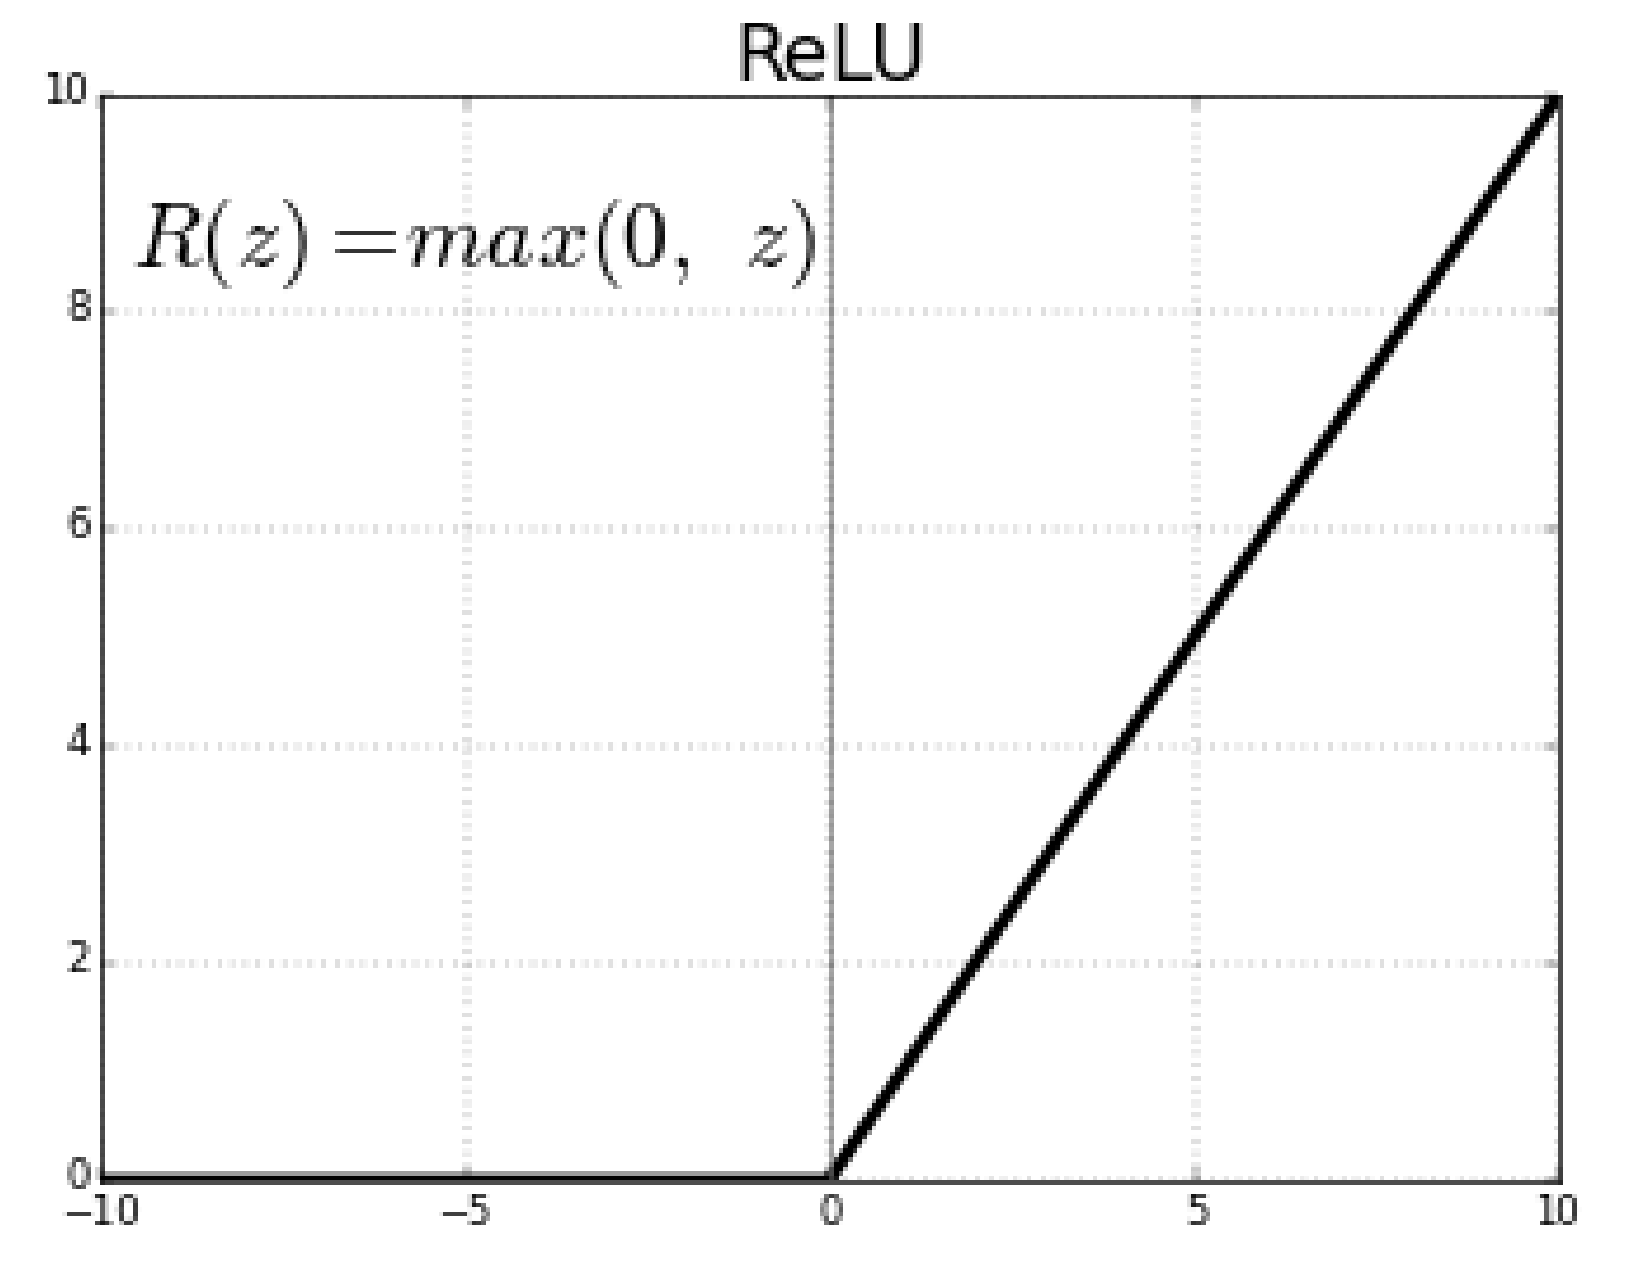
\includegraphics[scale=0.2]{FigurasUV/relu.pdf}
  \caption{Función ReLU}
\end{figure}

\end{frame}

\subsection{Ejemplo}
\begin{frame}{Funciones de activación}
Para entenderlo mejor, veamos un ejemplo:

\begin{figure}[h!]
  \centering
  
\includegraphics[scale=0.35]{FigurasUV/GOT.pdf}
  \caption{GOT}
\end{figure}

\end{frame}

\begin{frame}{Funciones de activación}
Los que han visto esta serie recordarán esta situación (spoiler):

\begin{figure}[h!]
  \centering
  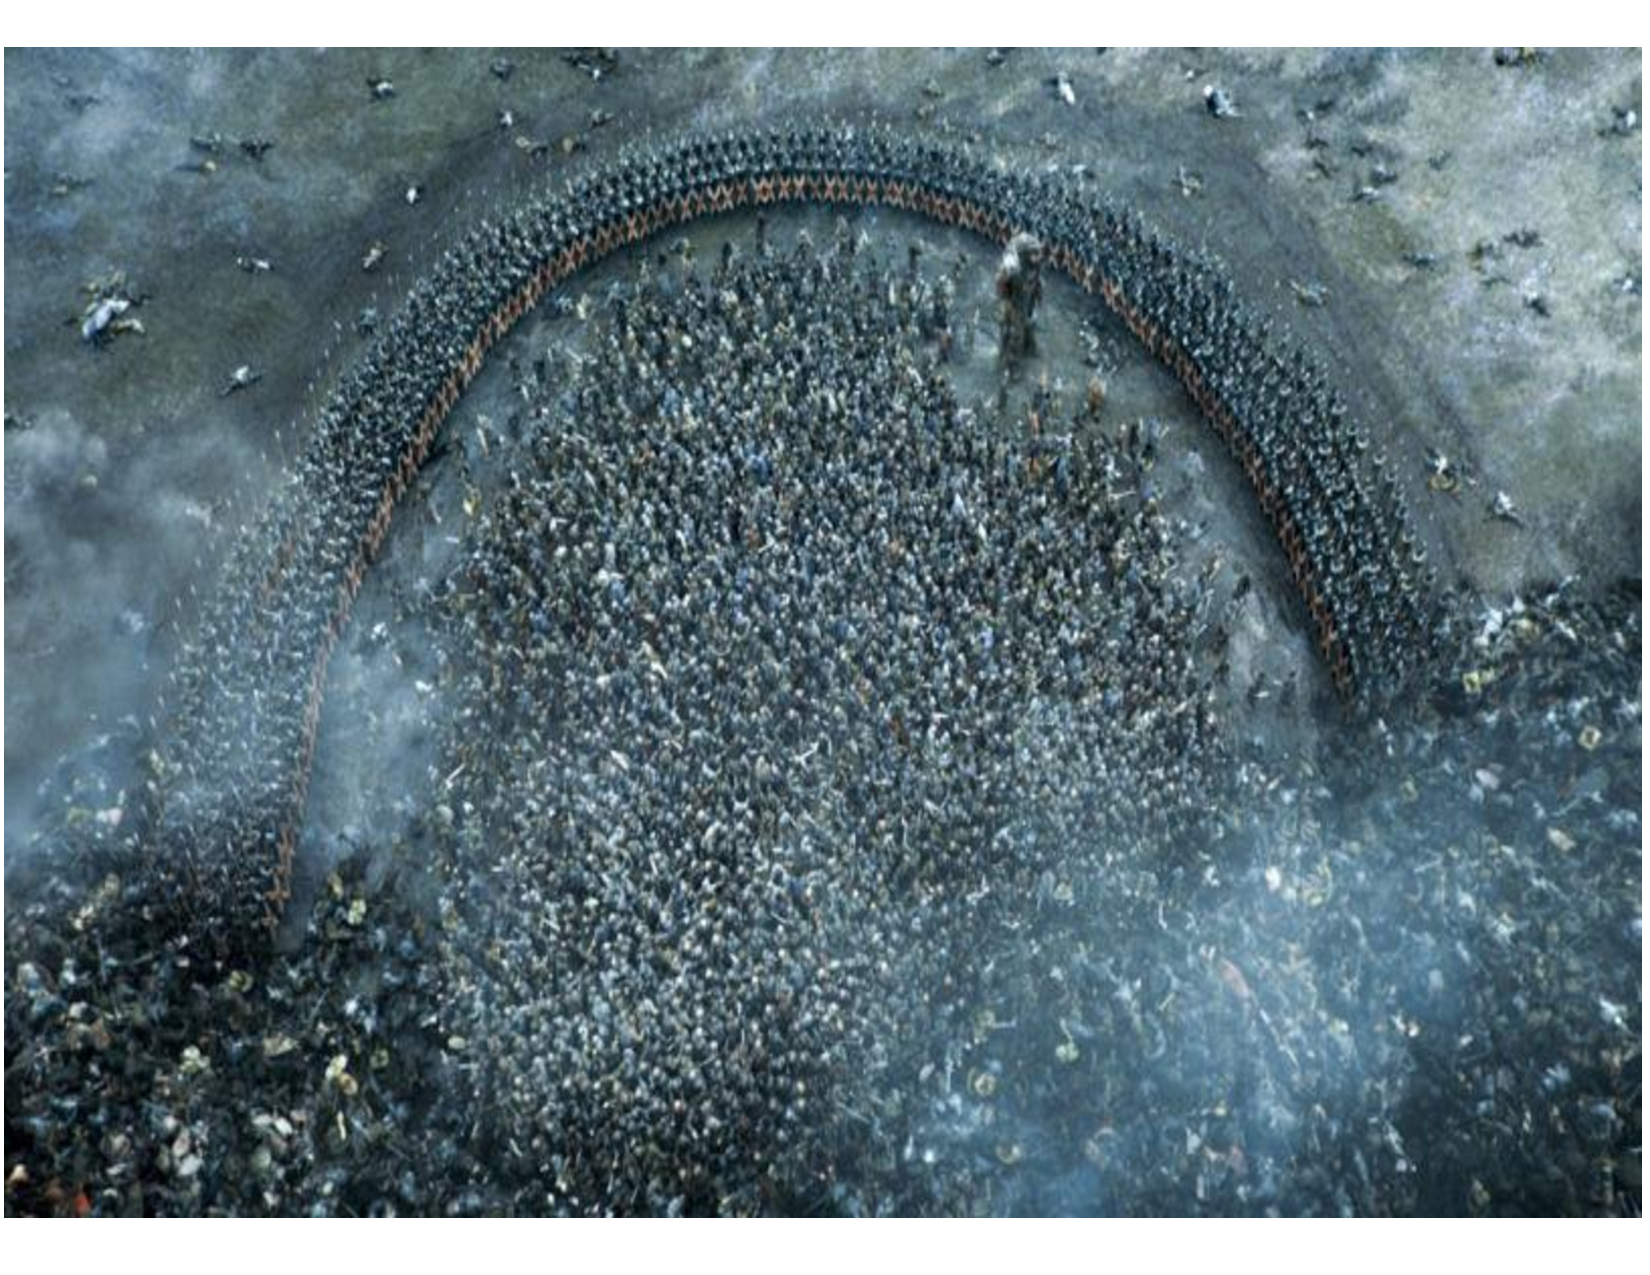
\includegraphics[scale=0.35]{FigurasUV/GOT1.pdf}
  \caption{GOT}
\end{figure}

\end{frame}

\begin{frame}{Funciones de activación}
Separando los ``buenos'' de los ``malos''.

\begin{figure}[h!]
  \centering
  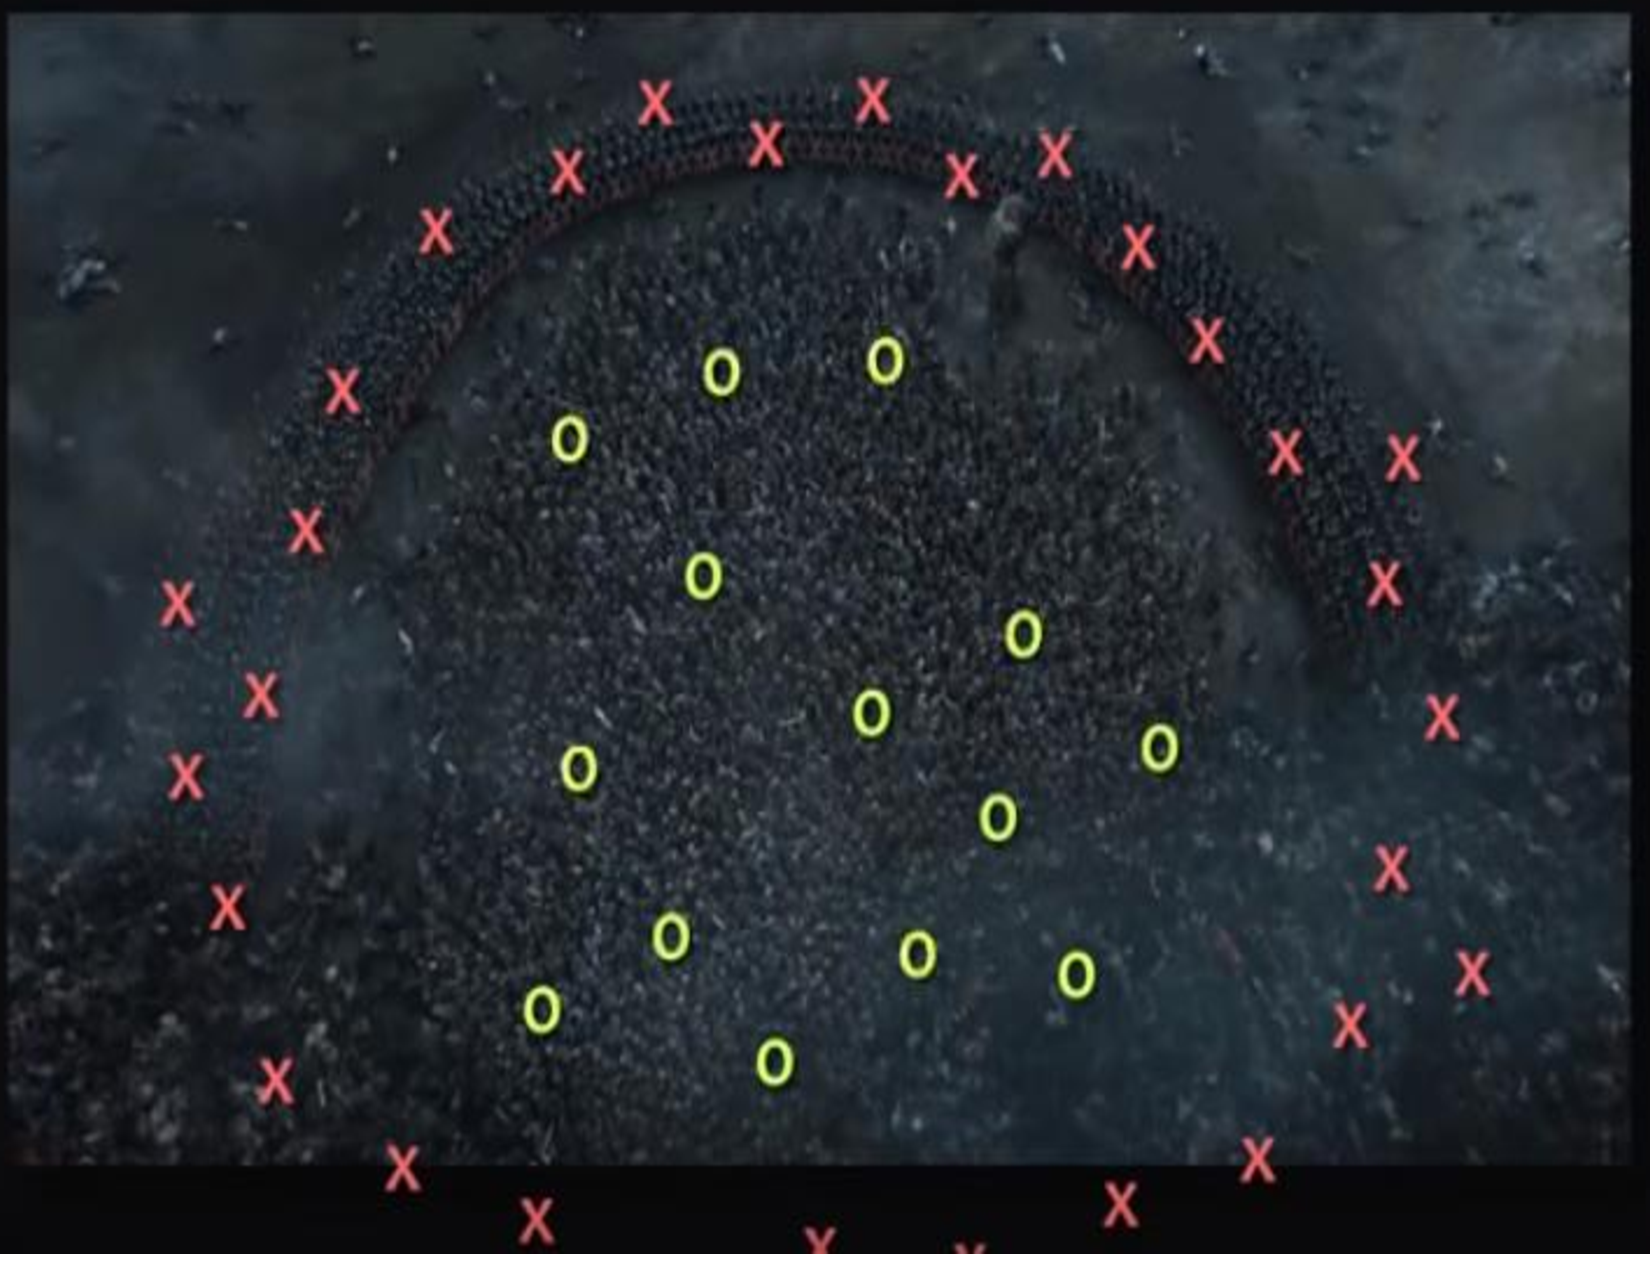
\includegraphics[scale=0.35]{FigurasUV/GOT2.pdf}
  \caption{GOT}
\end{figure}

\end{frame}

\begin{frame}{Funciones de activación}
Para intentar salvar a Jon Snow y a sus amigos utilizando una red neuronal, debemos resolver el problema de separar ambas nubes de puntos.

\begin{figure}[h!]
  \centering
  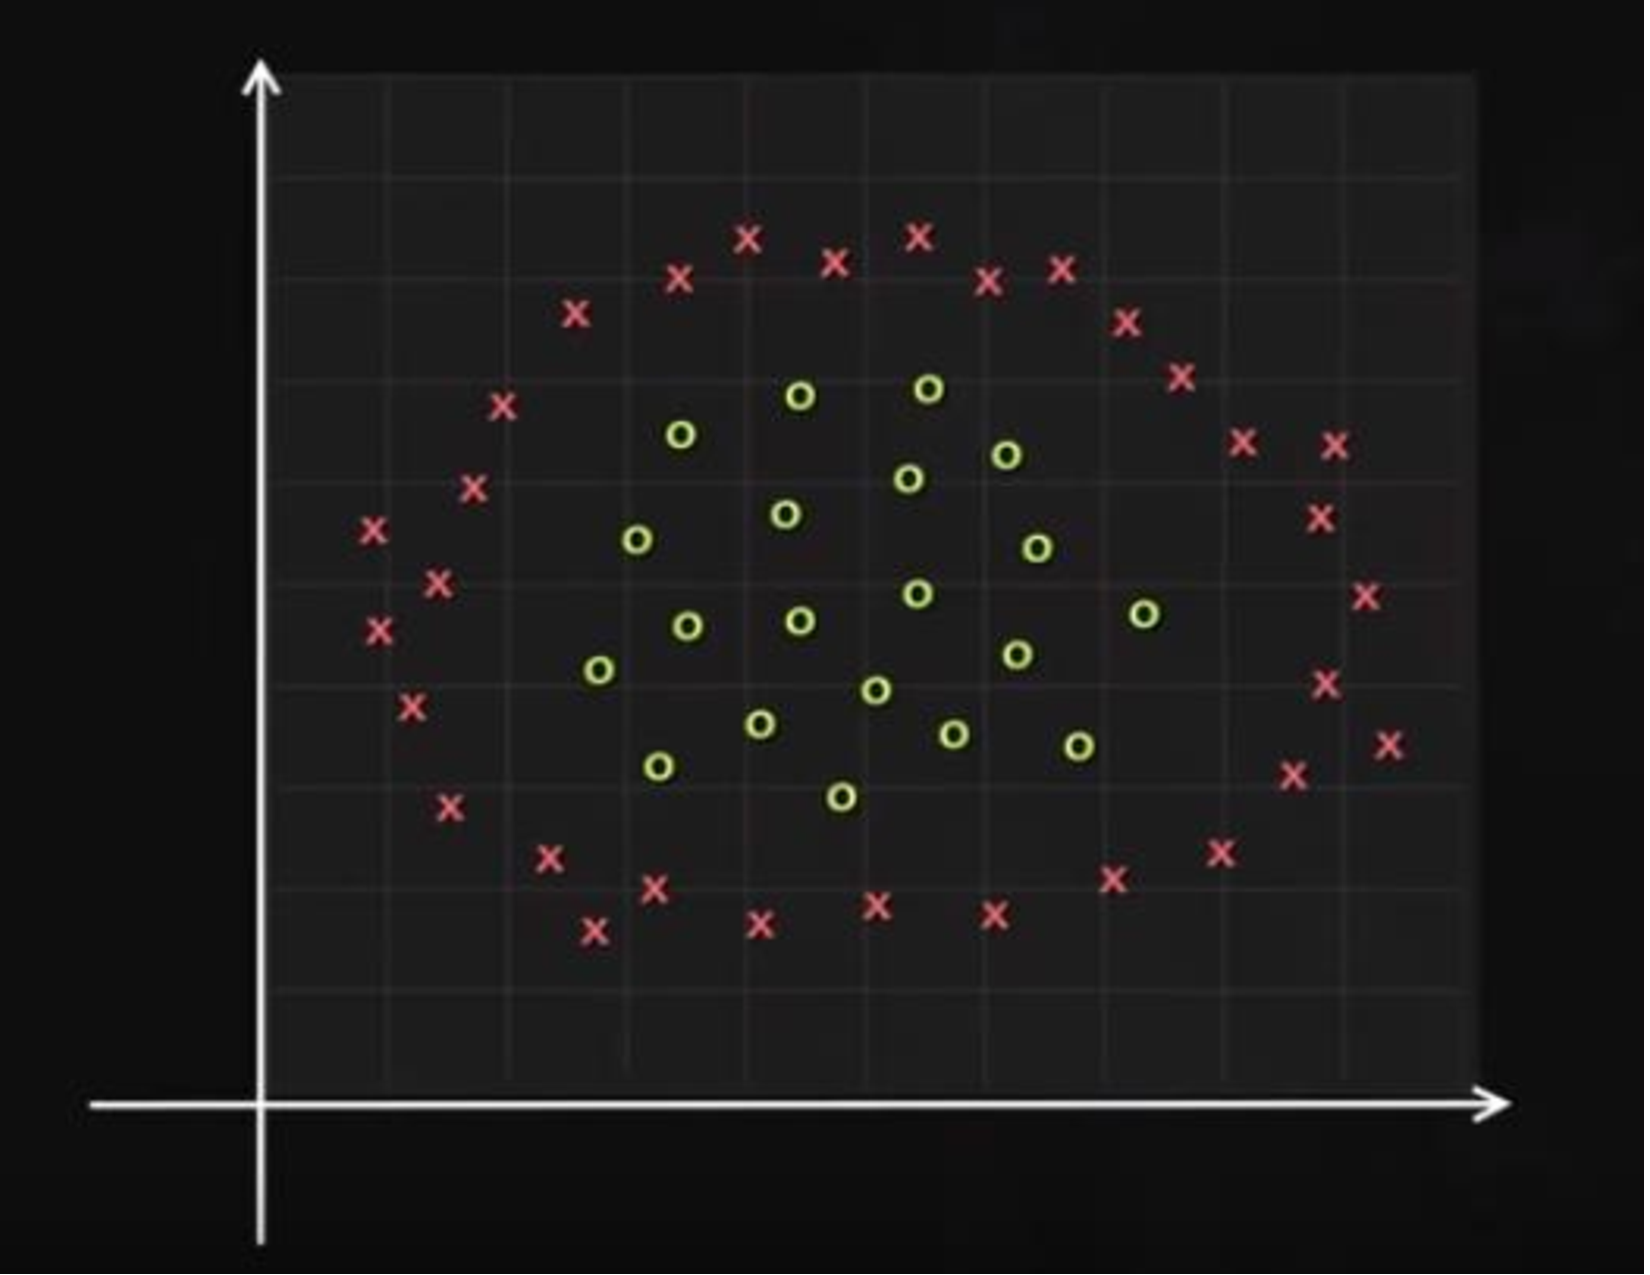
\includegraphics[scale=0.35]{FigurasUV/GOT3.pdf}
  \caption{GOT}
\end{figure}

\end{frame}

\begin{frame}{Funciones de activación}
En la vida real, este problema es similar al de diferenciar en una imagen células cancerígenas de las que no lo son.

\begin{figure}[h!]
  \centering
  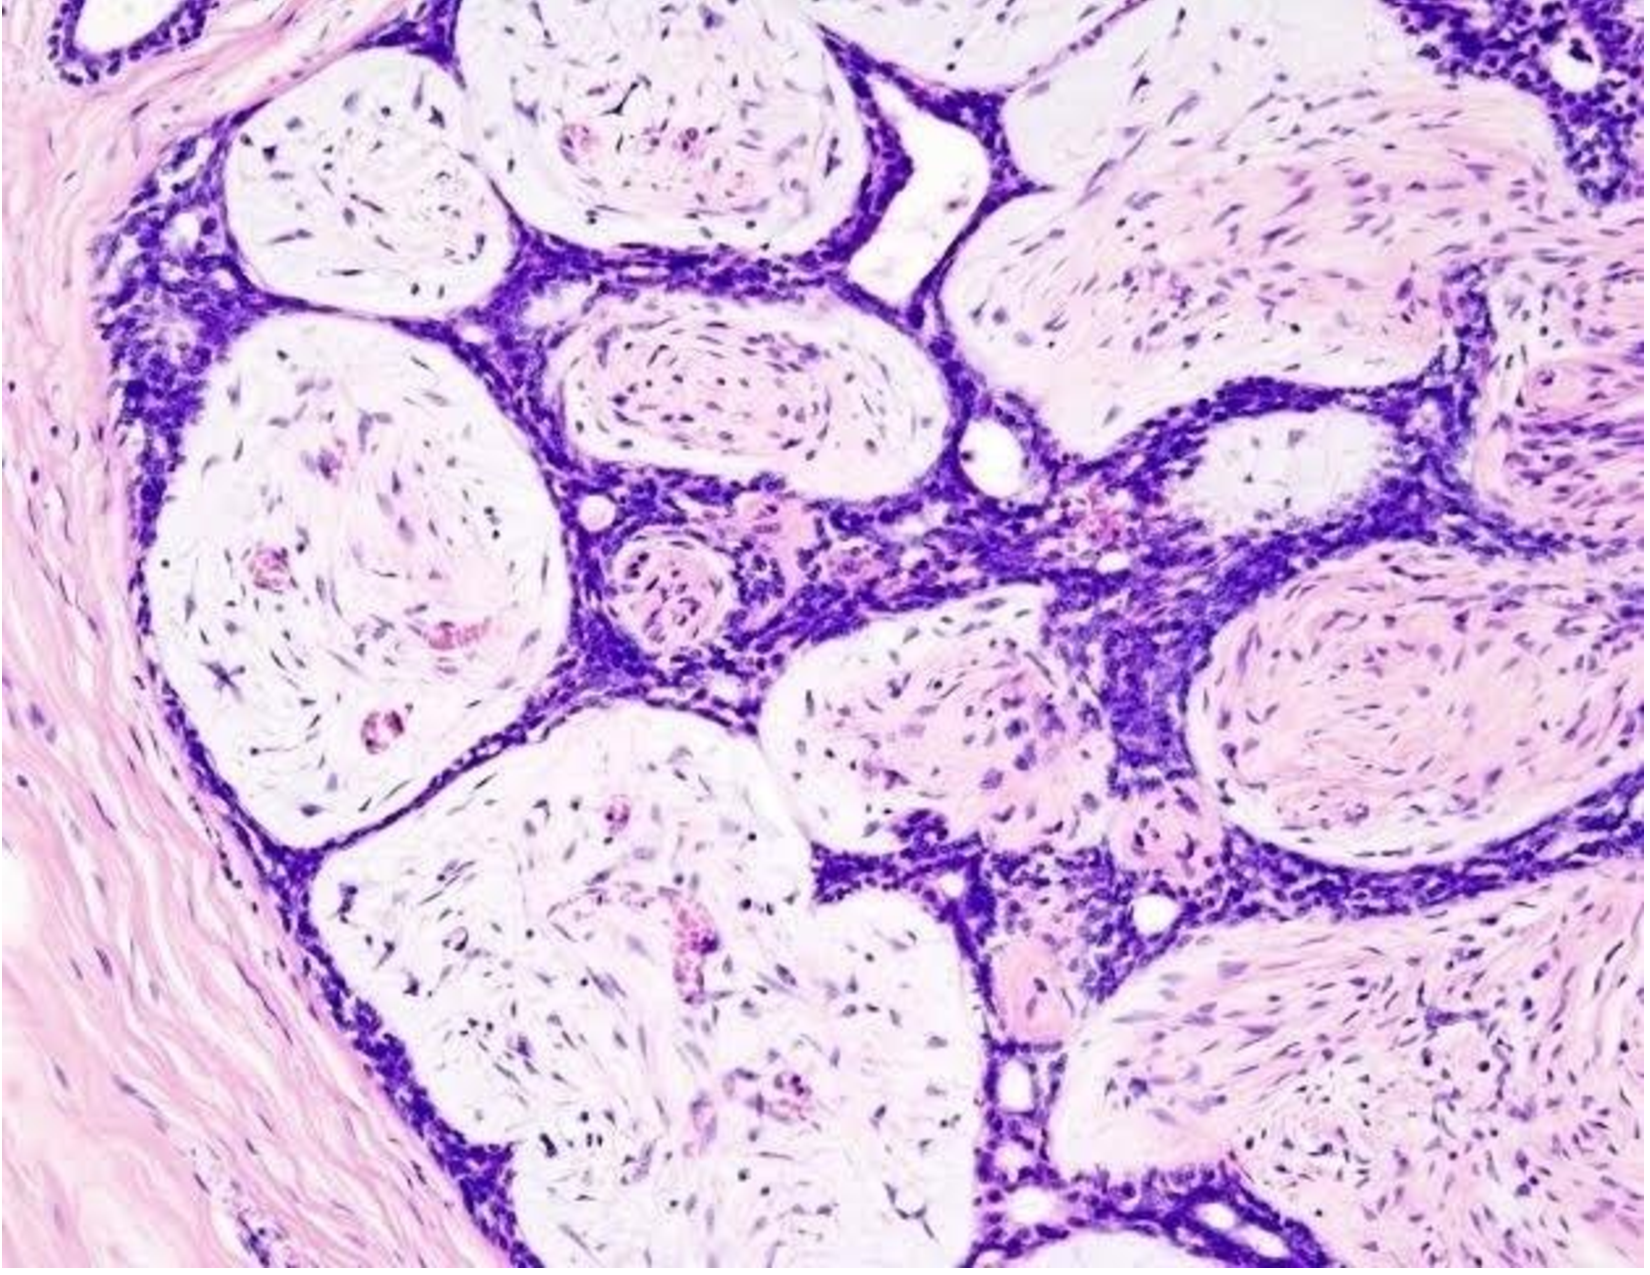
\includegraphics[scale=0.35]{FigurasUV/GOT4.pdf}
  \caption{GOT}
\end{figure}

\end{frame}

\begin{frame}{Funciones de activación}
De forma geométrica, una red neuronal utiliza las funciones de activación para separar nubes de puntos.

\begin{figure}[h!]
  \centering
  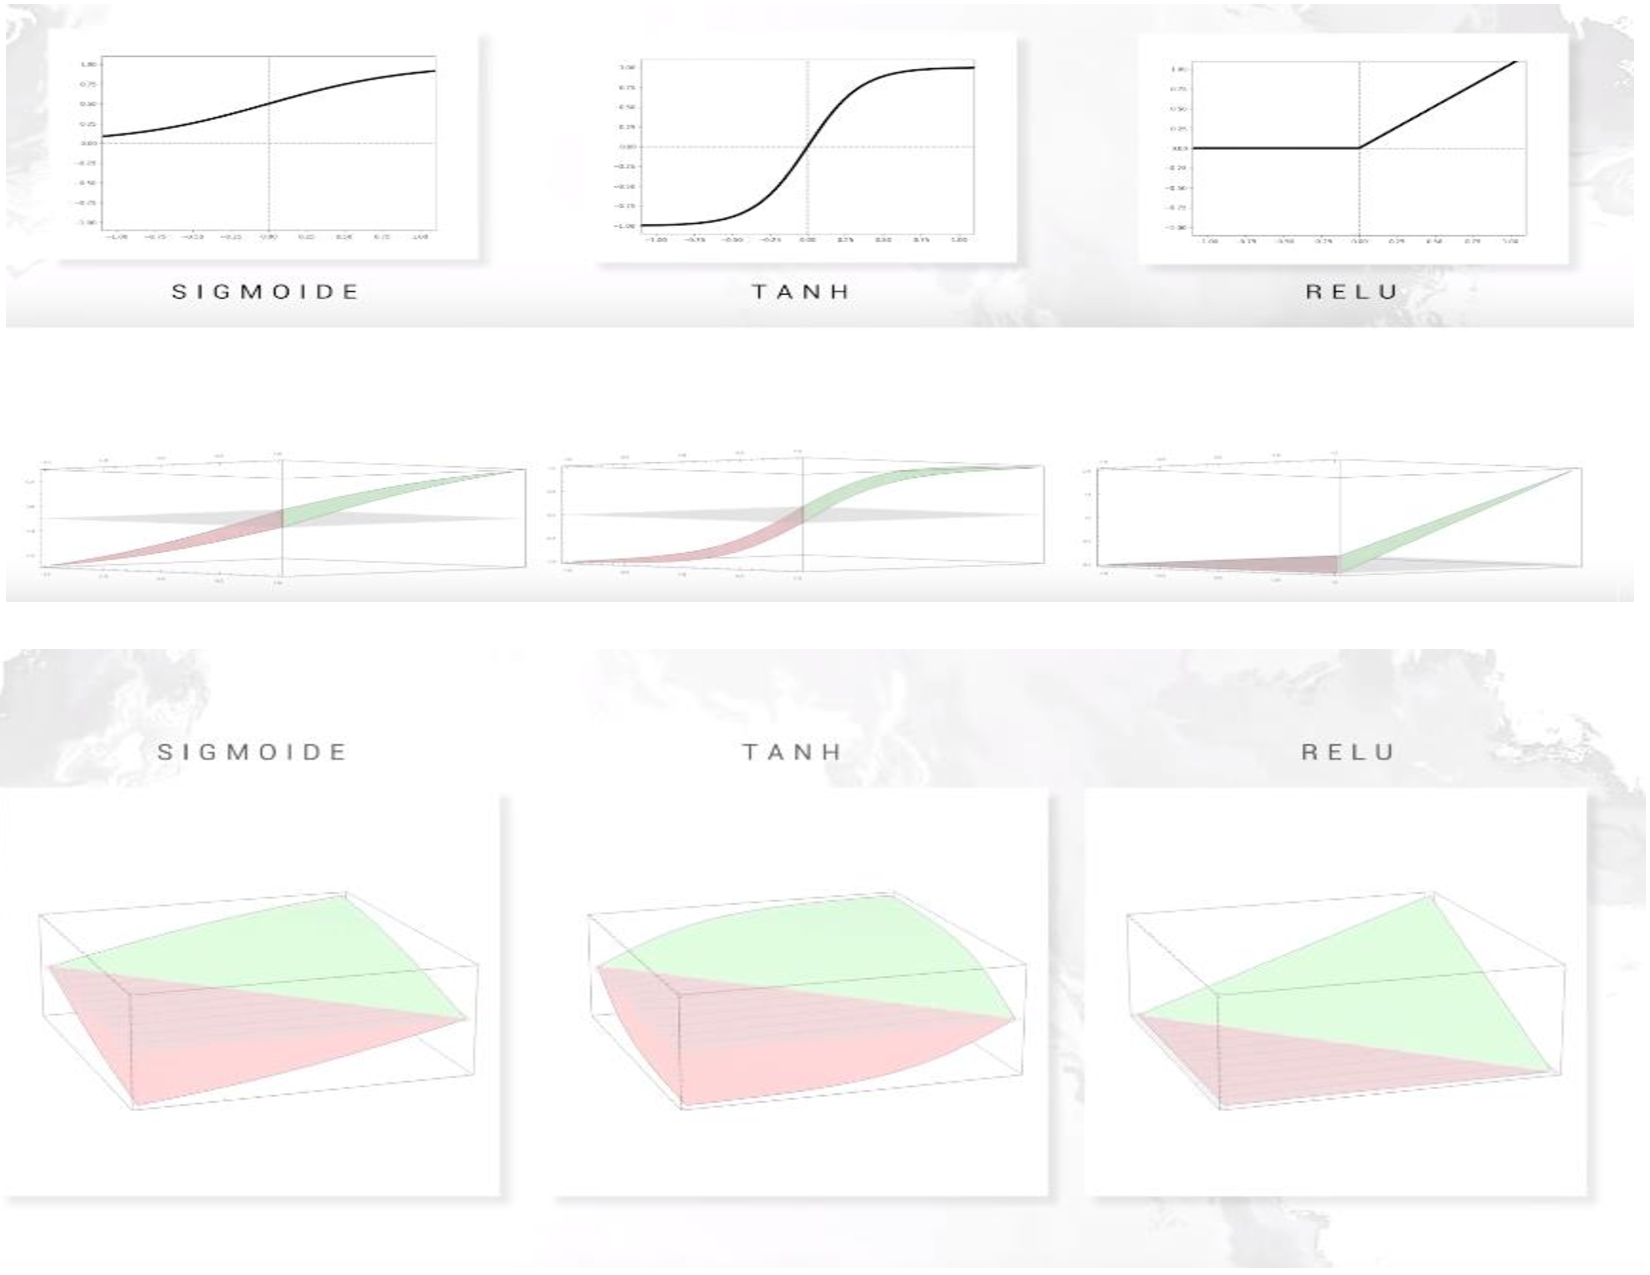
\includegraphics[scale=0.35]{FigurasUV/GOT5.pdf}
  \caption{GOT}
\end{figure}

\end{frame}

\begin{frame}{Funciones de activación}
Esto se logra combinando varias neuronas; en nuestro problema particular encadenamos varias neuronas con funciones de activación sigmoide, cada una con orientación distinta. 

\begin{figure}[h!]
  \centering
  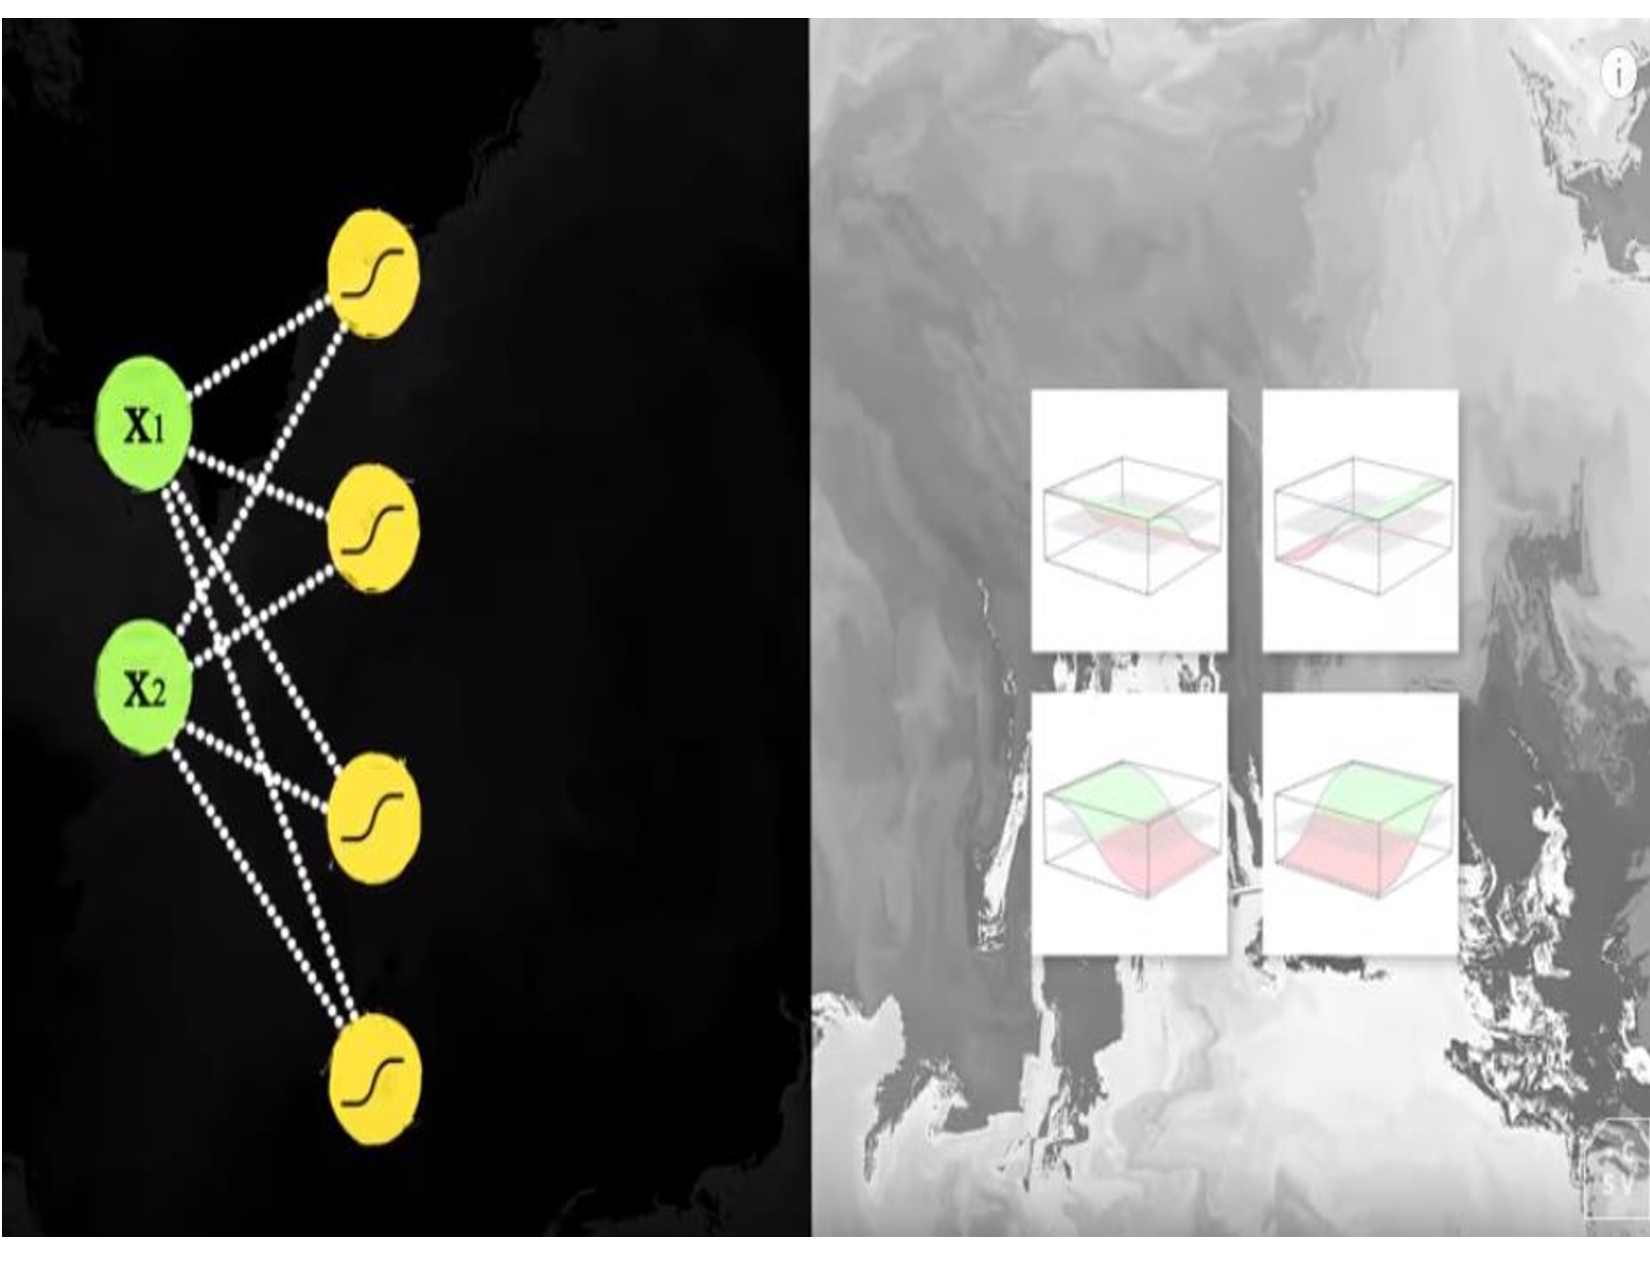
\includegraphics[scale=0.30]{FigurasUV/GOT6.pdf}
  \caption{GOT}
\end{figure}


\end{frame}

\begin{frame}{Funciones de activación}
Al unir estas neuronas obtenemos la forma que separa las dos nubes de puntos, una superficie plana con un bulto en medio.


\begin{figure}[h!]
  \centering
  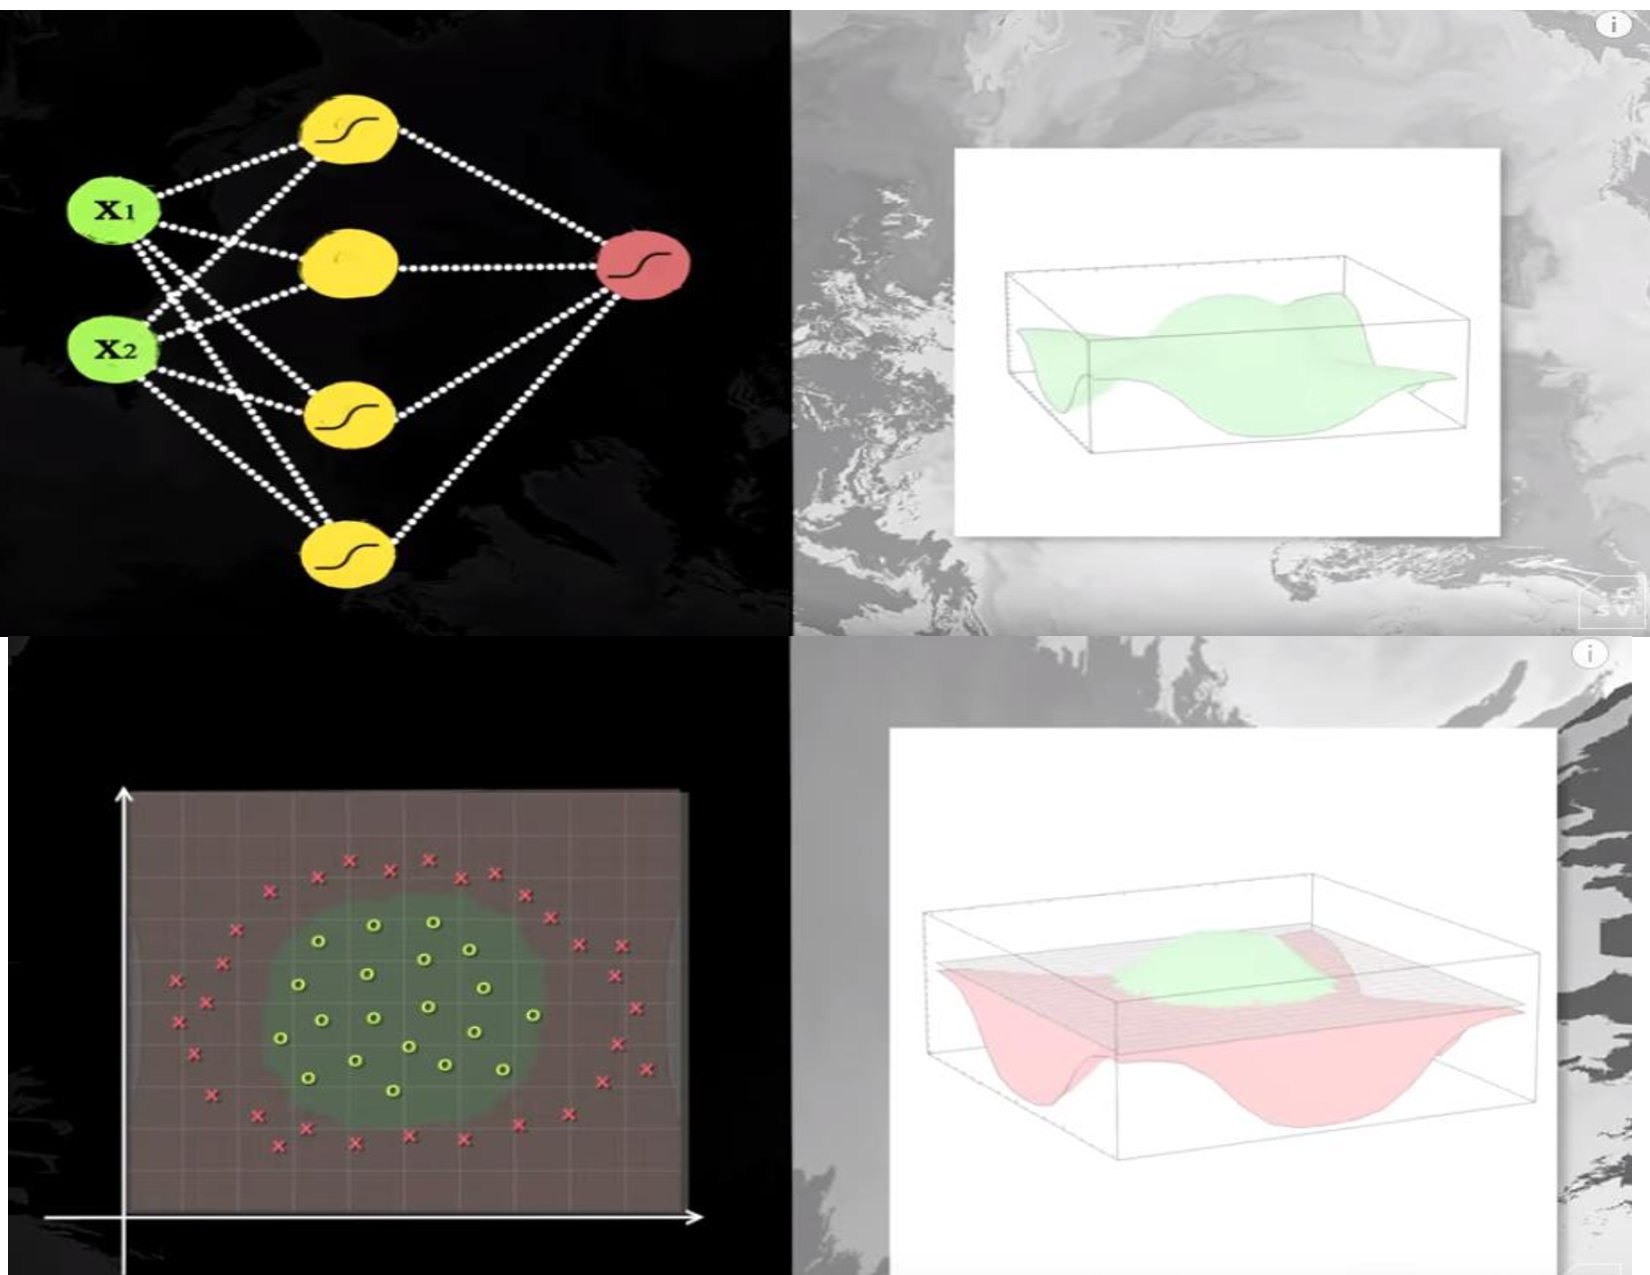
\includegraphics[scale=0.30]{FigurasUV/GOT7.pdf}
  \caption{GOT}
\end{figure}

\end{frame}
\section{Gradient Descent}
\begin{frame}{Gradient Descent}
Para entender de forma intuitiva este algoritmo imaginemos que estamos en la punta de una montaña y queremos descender al punto más bajo, sin embargo vamos con los ojos vendados, lo más lógico es ir tanteando la inclinación del terreno y desplazarnos por donde la pendiente descienda con mayor intensidad, los pasos a seguir serían evaluar la inclinación para conocer la dirección con la mayor pendiente, luego caminamos una distancia en dicha dirección y
nos detenemos, volvemos a repetir hasta llegar a un lugar plano.
\end{frame}

\begin{frame}{Gradient Descent}
\begin{figure}[h!]
  \centering
  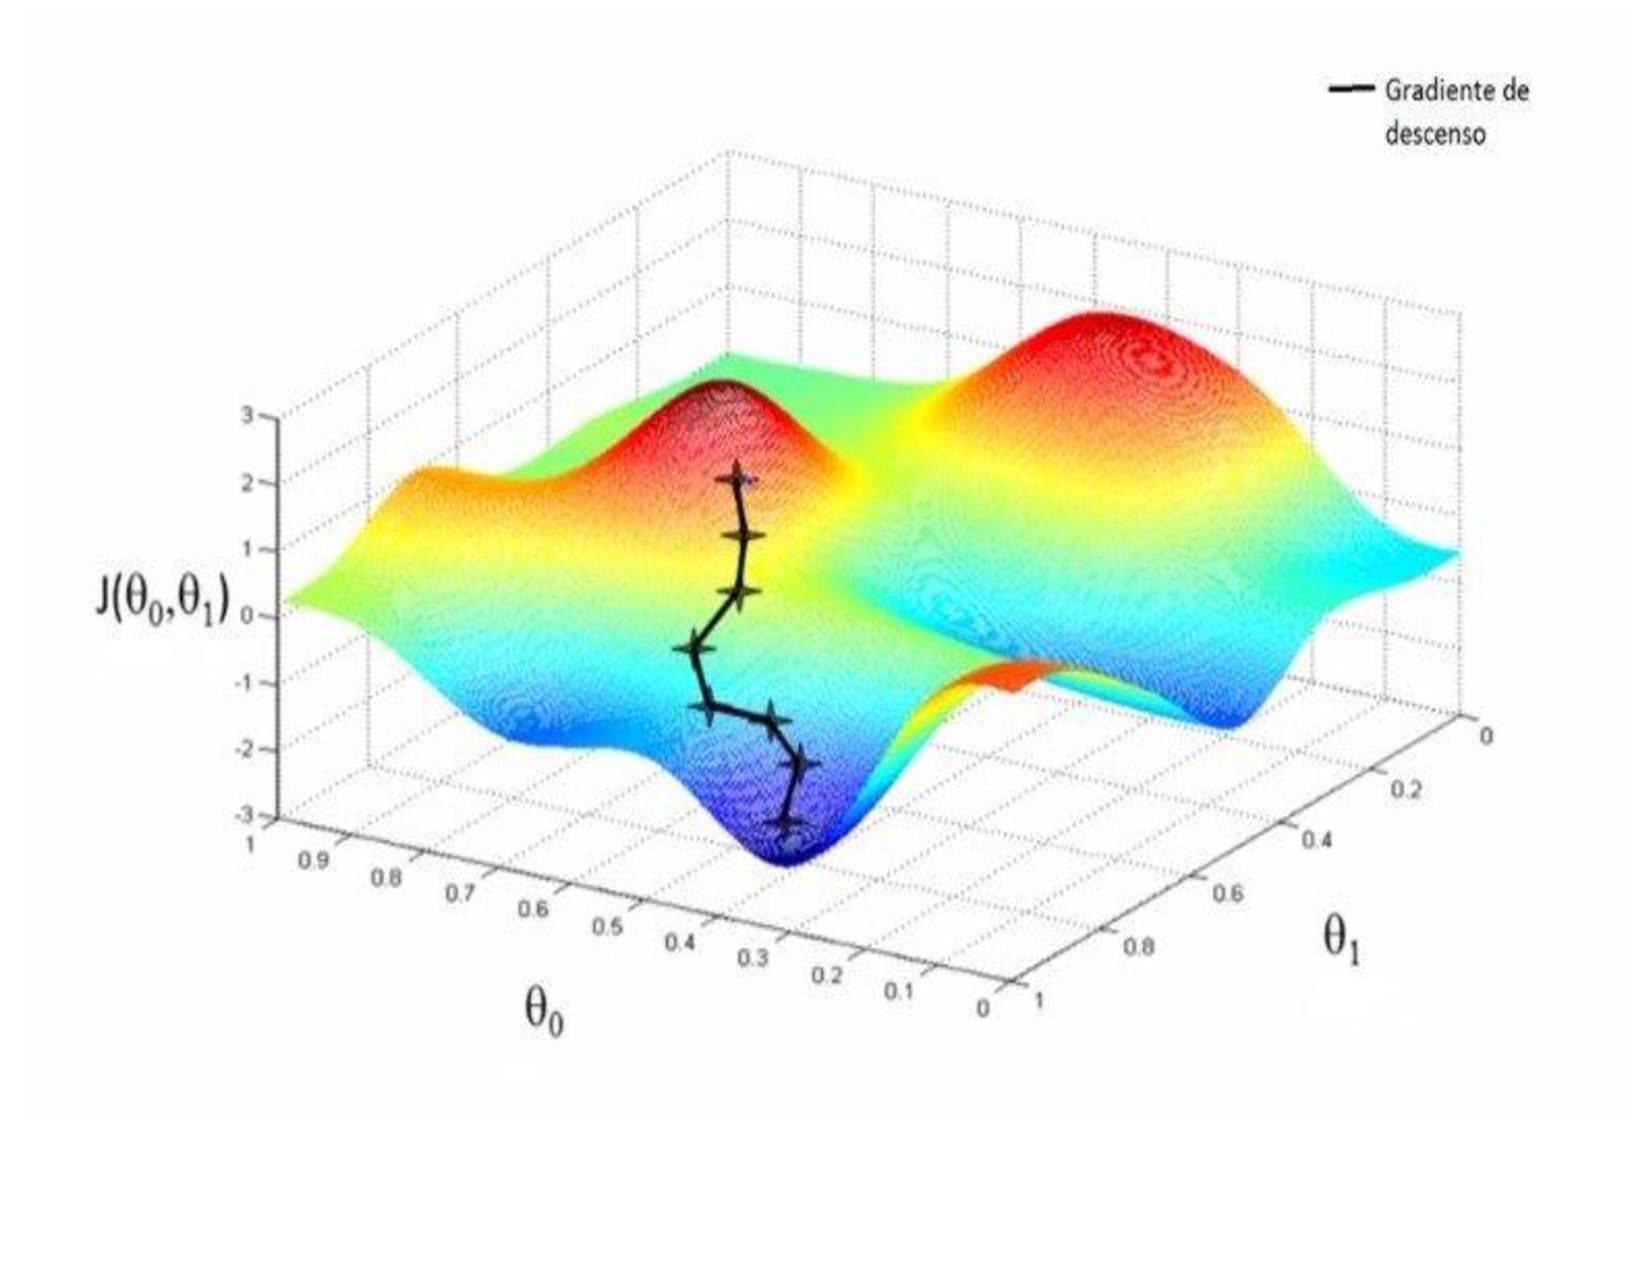
\includegraphics[scale=0.33]{FigurasUV/GD.pdf}
  \end{figure}
\end{frame}

\begin{frame}{Gradient Descent}
Matemáticamente, esto seria calcular las derivadas de la funcion de coste para cada parámetro en un punto aleatorio, estos nos dirá la pendiente en ese punto para cada parámetro, el vector de estas derivadas se denomina vector gradiente $\triangledown W$ y nos indica la dirección hacia la que la pendiente asciende, pero como lo que queremos es descender, es lógico trabajar con $-\triangledown W$ la dirección contraria, nos desplazamos en esa dirección y repetimos el proceso, calculamos las derivadas parciales para el nuevo punto y volvemos a movernos iterativamente hasta llegar a un punto donde movernos no suponga una variación notable en el coste, es decir que la pendiente sea próxima a nula.

\end{frame}

\begin{frame}{Gradient Descent}
El algoritmo del descenso del gradiente lo podemos denotar como $\theta:=\theta-\alpha\nabla W$ donde $\theta$ es mi parámetro el cual se va a actualizar y $\alpha$ es el  ratio de aprendizaje. 

\begin{figure}[h!]
  \centering
  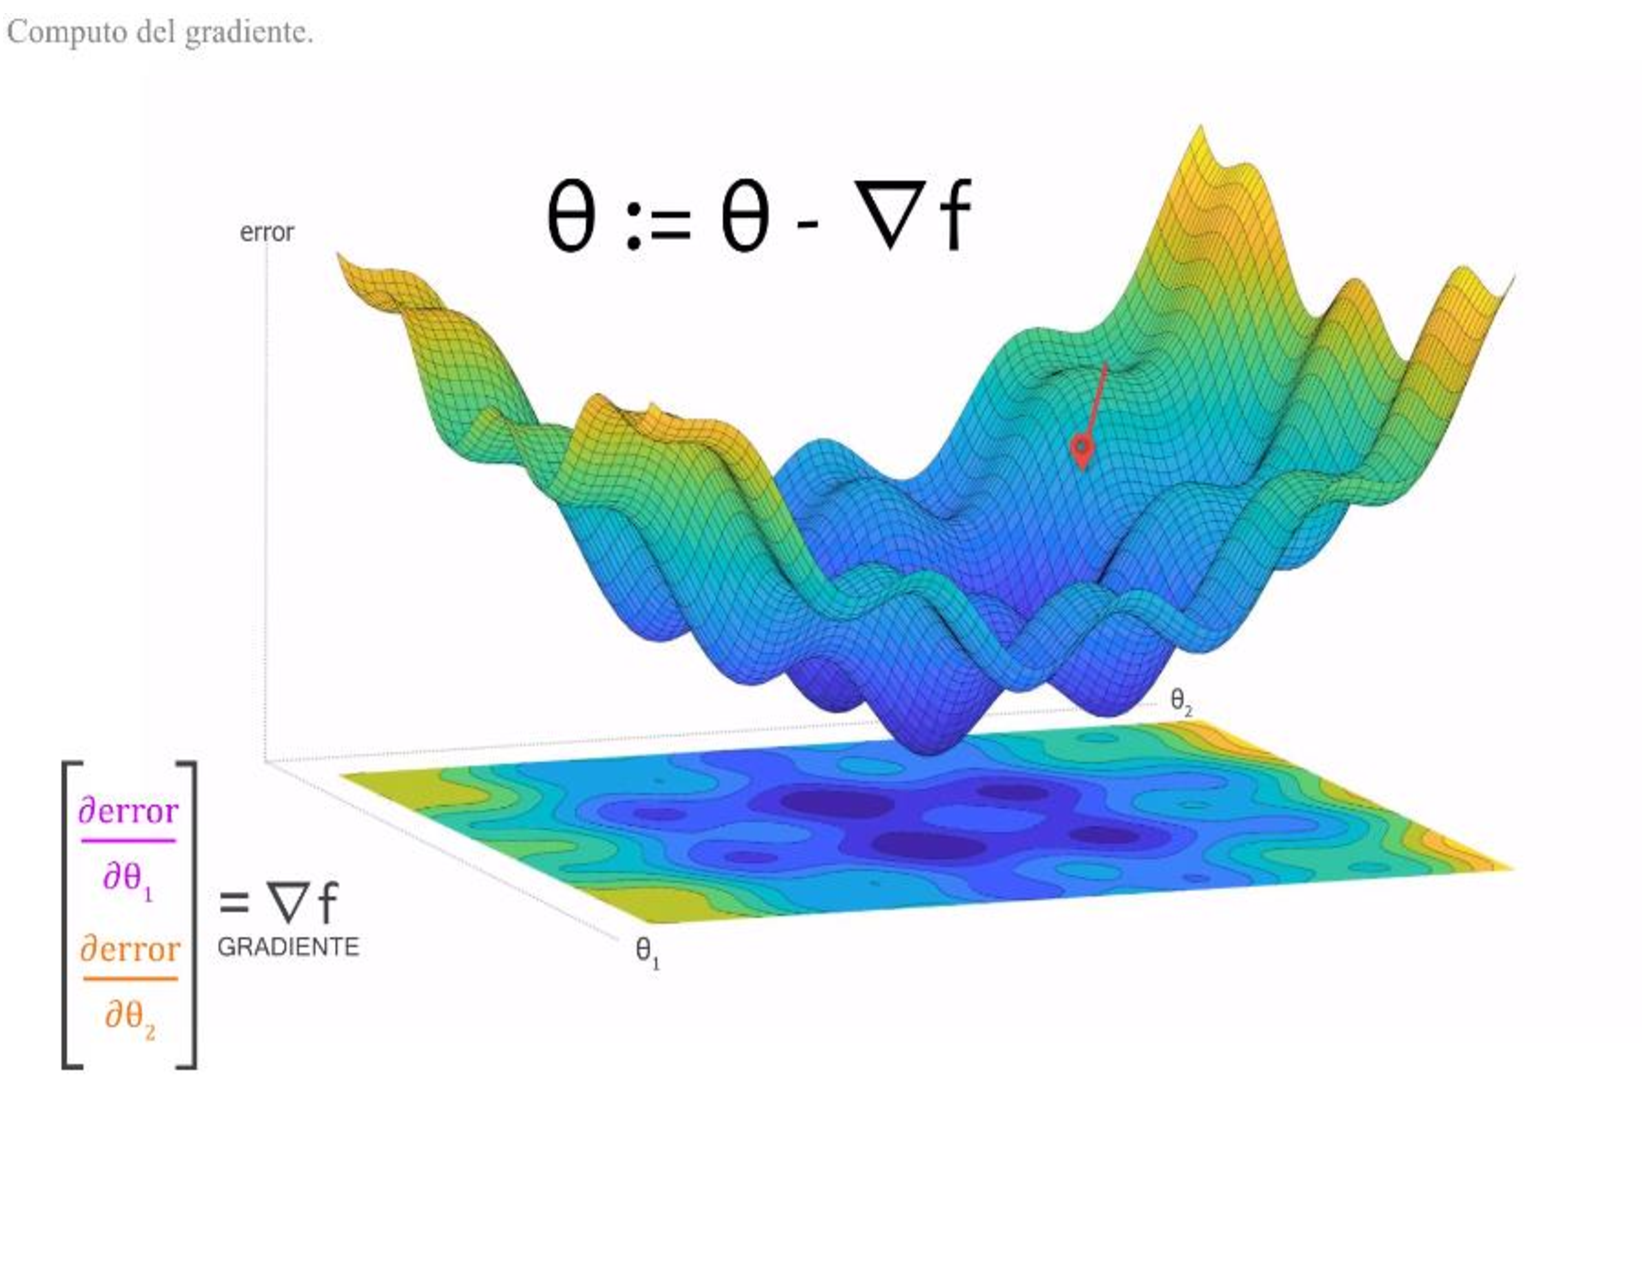
\includegraphics[scale=0.33]{FigurasUV/GD1.pdf}
  \caption{Gradient Descent}
\end{figure}
 
\end{frame}


\section{Backpropagation}
\begin{frame}{Backpropagation}
El algoritmo de Backpropagation sirve para conocer qué error le corresponde a cada una de las neuronas en una red neuronal. Para hacer uso del descenso del gradiente es necesario conocer un vector gradiente y este solo se consigue conociendo la función de coste asociada.


\end{frame}

\begin{frame}{Backpropagation}
Pensemos en la siguiente cadena de responsabilidades.

\begin{figure}[h!]
  \centering
  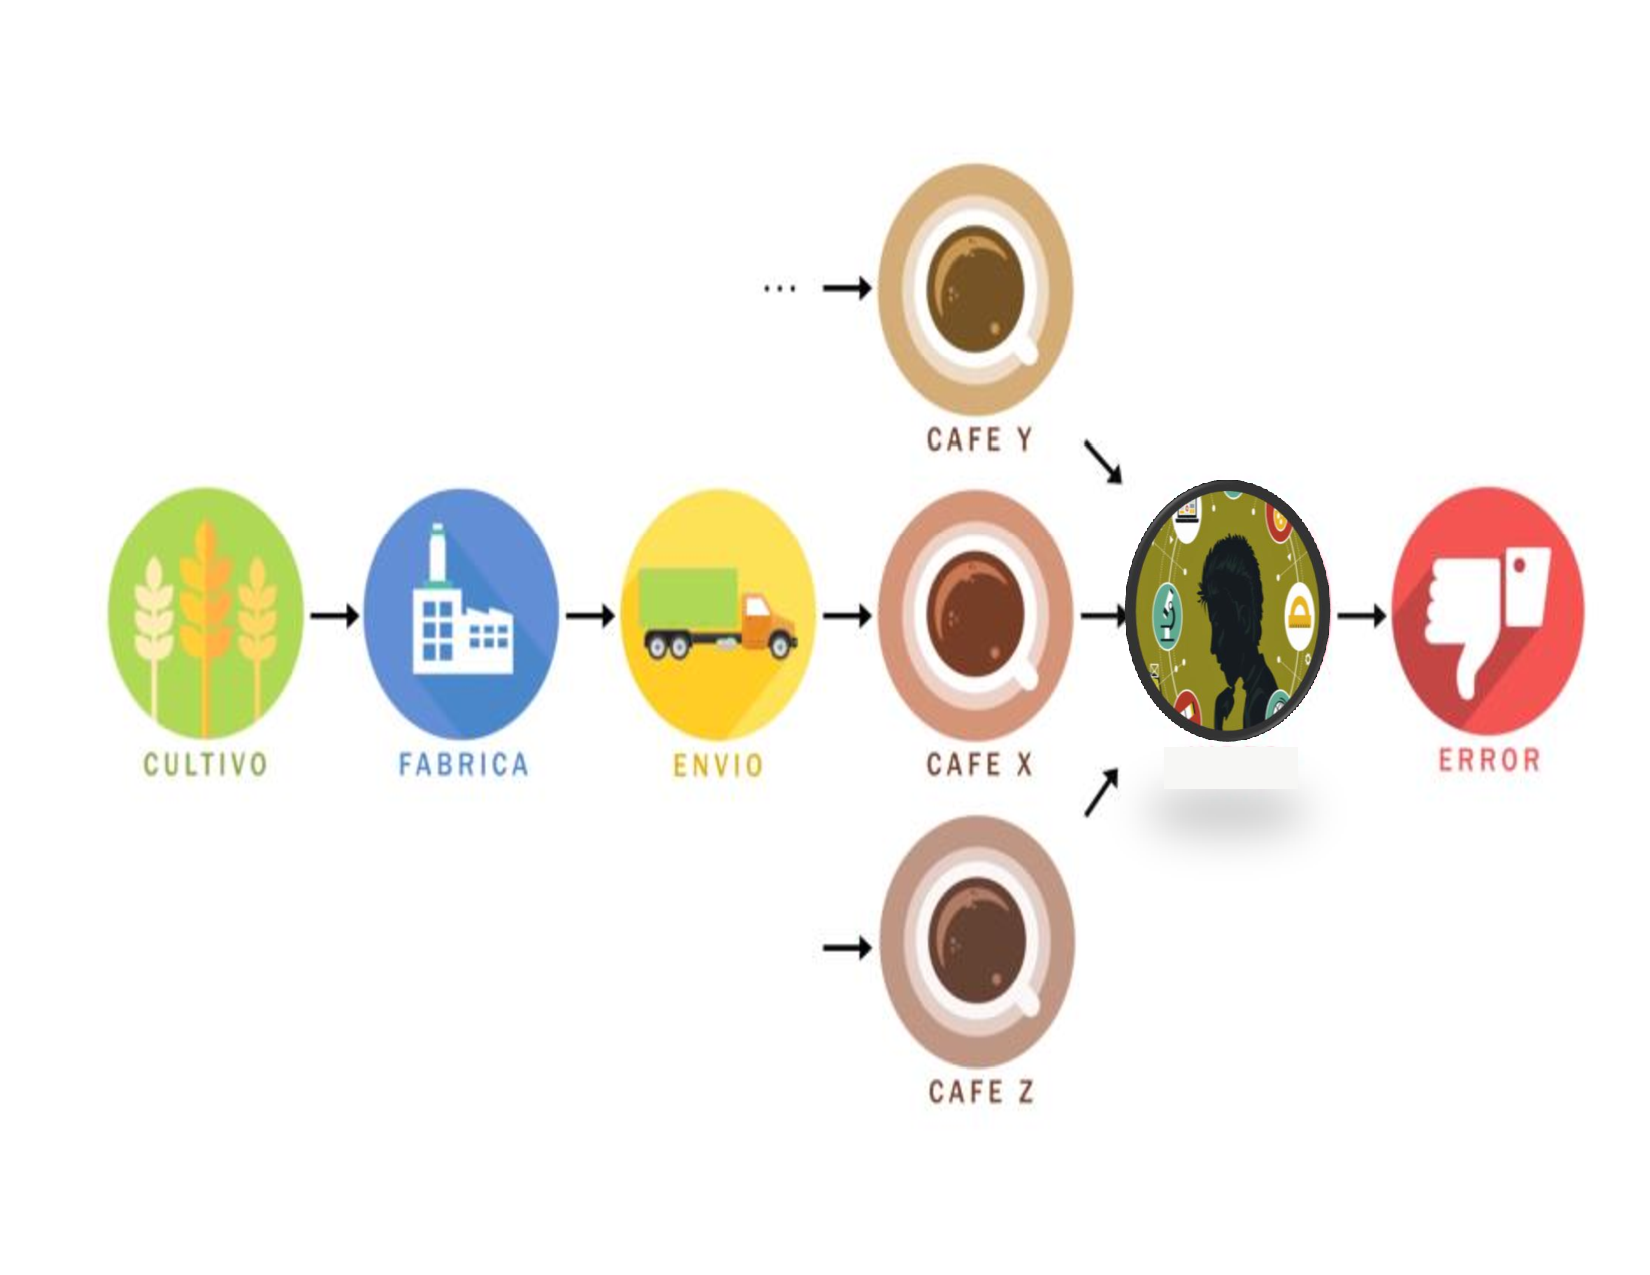
\includegraphics[scale=0.34]{FigurasUV/BP.pdf}
  \caption{Cadena de responsabilidades}
\end{figure}


\end{frame}

\begin{frame}{Backpropagation}

Esta cadena de responsabilidades se puede asemejar a una red neuronal donde cada nodo es una neurona con una tarea determinada, el examen es el resultado de salida o Output layer y la evaluación que obtenemos la podemos ver como nuestra función de coste, así, ese resultado desfavorable en el examen genera una fuerte señal de error, lo que se hace es analizar toda la cadena de responsabilidades que ha afectado el resultado y si encontramos una neurona que tuviera influencia en el error obtenido, entonces debemos responsabilizarla con parte de ese error, este análisis debe realizarse hacia atrás, desde la señal de error hacia las primeras capas y esto es así, ya que en una red neuronal el error de las capas anteriores depende del error de las capas posteriores, por ejemplo si nos damos cuenta que el resultado del examen no depende mucho de si la calidad del café es buena o mala, entonces el error en las fases anteriores, como el método de molido o el método de cosechado también afectan poco al error final. 

\end{frame}

\begin{frame}{Backpropagation}

Con el algoritmo de Backpropagation obtenemos el error que tiene cada neurona en el error final, y con esto, podemos utilizar el descenso del gradiente para minimizar el error en cada una de las neuronas como si se tratara de una única regresión.

~\\Estos algoritmos se pueden escribir de forma que:

$$\nabla W^{k}=\frac{1}{n}\sum_{i=1}^{n}\frac{\delta L[y_i,f(x_i;W)]}{\delta W^{k}}$$

$$W^{k}:=W^{k}-\alpha\nabla W^{k}$$
\end{frame}

\section{Conclusiones}
\begin{frame}{Conclusiones}
Podemos decir que aunque su funcionamiento es complejo y en algunos casos abstracto, las redes neuronales son útiles para resolver problemas en muchas áreas del conocimiento y la tecnología, automatizando procesos, logrando replicar comportamientos inteligentes y dando cabida a un mundo de posibilidades.

\begin{itemize}
\item[1.] Las funciones de activación resuelven el problema de la linealidad dentro de las redes neuronales de manera optima, dando soluciones a problemas complejos que no son fáciles de modelar con regresiones lineales

\item[2.] EL algoritmo del descenso del gradiente y backpropagation cumplen una función importante en la anatomía de una red neuronal, ya que son el centro del aprendizaje de la misma.

\item[3.]Las redes neuronales son capaces de modelar comportamientos tan abstractos, que muchas de estas son completas cajas negras, y logran encontrar relaciones o asociaciones entre variables las cuales un humano no imaginaría.

\end{itemize}
\end{frame}


\section{Bibliografía}
\begin{frame}
  \frametitle{Bibliografía}
  
\nocite{L,EyH,Y}
  
  \bibliographystyle{plain}
  \bibliography{references}
\end{frame}


\end{document}
